% !TeX encoding = UTF-8
% !TeX program = pdflatex
% !TeX spellcheck = en_US

\documentclass[LaM,binding=0.6cm]{sapthesis}
\usepackage{float}
\usepackage{microtype}

\usepackage{hyperref}
\hypersetup{pdftitle={Arrhythmia classification from ECG signals},pdfauthor={Angelo Catalani}}

% Remove in a normal thesis
\usepackage{lipsum}
\usepackage{curve2e}
\definecolor{gray}{gray}{0.4}
\newcommand{\bs}{\textbackslash}

% Commands for the titlepage
\title{Arrhythmia classification from ECG signals}
\author{Angelo Catalani}
\IDnumber{1582230}
\course{Engineering in Computer Science}
\courseorganizer{Dipartimento di Informatica, Automazione e Gestionale}
\AcademicYear{2018/2019}
\copyyear{2013}
\advisor{Prof. Aris Anagnostopoulos}
\coadvisor{Prof. Ioannis Chatzigiannakis}
\authoremail{catalaniangelo@gmail.com}

\examdate{15 July 2019}
\examiner{Prof. Nome Cognome}
\examiner{Prof. Nome Cognome}
\examiner{Dr. Nome Cognome}
\versiondate{\today}



\begin{document}

\frontmatter

\maketitle

\dedication{Dedicated to\\ my parents}

\begin{abstract}
A programmer is a problem solver and its activity requires a high level of creativity as well as multidisciplinary knowledge.\\This project gave me the opportunity to implement innovative algorithms for medical purposes: I strongly believe in technological advancement as the key to improve the quality of life and world around us.
\end{abstract}

\begin{acknowledgments}
I would like to express my special thanks of gratitude to my professors (Aris Anagnostopoulos and Ioannis Chatzigiannakis) who gave me the golden opportunity to do this wonderful project.\\Secondly, I would also like to thank my parents and relatives who sustained me a lot over my studies.
\end{acknowledgments}

\tableofcontents

\listoffigures

\mainmatter

\chapter{Introduction}
Cardiovascular diseases (CVDs) are the first cause of death worldwide: 18 million people died from CVDs in 2016, representing 31\% of all global deaths (\cite{who}).\\This project is focused on the cardiovascular diseases related to complications with the electrical system that regulates the steady heartbeat and generates abnormal heartbeats called arrhythmias.\\A great deal of people, during life, can experience irregular heartbeats and generally,  they are harmless and happen in healthy people free of heart disease.\\However, some abnormal heart rhythms can be serious or even deadly.\\A standard tool to diagnose arrhythmias is the electrocardiogram (ECG): measurement of the heart's electrical activity.\\Since it is a non-invasive and painless test for the patients, it can be employed to collect massive volumes of data, and subsequently analyze them, with the purpose of automatically detecting arrhythmias.\\The equipment to produce electrocardiograms is principally present in hospitals, where cardiologists use their knowledge and experience to carefully evaluate the ECG. However, this activity is time-consuming and prone to error: an automatic approach can support them during their decision.\\In addition to this, accurate and low-cost diagnosis of arrhythmic heartbeats is highly desirable since it can detect early heart problems and prevent dangerous consequences. This is the reason it is not surprising recent literature is focused on this topic.\\In general, the ECG's analysis is constituted of two phases:
\begin{enumerate}
\item beat detection: extrapolate the temporal segment of the ECG related to the contraction of the heart
\item arrhythmia  classification: detection of arrhythmic beats
\end{enumerate} 
This work is concentrated only on the latter, that is more challenging because until now, there is not any perfect solution to the problem.\\We propose a series of algorithms able to automatically detect arrhythmias, with the aim for the future, to implement them on wearable devices.\\In detail, several works have proposed a complete infrastructure to integrate that devices in a fog-computing organization.\\Specifically, \cite{fog} and \cite{citf}, describe an environment with:
\begin{enumerate}
\item Wearable Device. It collects data from the ECG sensor and detects arrhythmias with suitable algorithms
\item Edge Device. It is patient's device with software to communicate with the wearable device and perform more complex computation
\item Cloud Services. They offer all the necessary features to facilitate authentication, notifications, data integration and other services relying on privacy-preserving data integration
\end{enumerate}
The described fog computing approach extends the cloud computing paradigm by migrating data-processing closer to the production site, thus accelerating the system's responsiveness to events (\cite{ufcf},\cite{ufcf2},\cite{fog}).\\This prototype will allow patients to share information to their physicians, monitor their health status independently and notify the authorities rapidly in emergency situations.\\Historical data will also be available for further analysis, towards identifying patterns that may improve medical diagnoses in the foreseeable future (\cite{otdo}).\\The performance of the system is evaluated concerning the accuracy of detecting abnormal events and the power consumption of the wearable device. Results indicate that a very high percentage of success can be achieved in terms of event detection ratio and the device being operative up to a several days without the need for a recharge (\cite{potf}, \cite{aoat}).\\We use the \textit{MIT-BIH Arrhythmia Database dataset}: it is open source and consists of 47 patient's ECG recording.\\Initially, we have investigated the literature about the pre-processing techniques to remove noise from the ECG and deal with unbalanced classes in the dataset: Discrete Wavelet Transform and Median Filter for de-noise; Smote, Adasyn for weighted loss (data augmentation).\\Secondly, we have tried a simple model based on Random Forest, and subsequently more complex.\\In particular, we have re-implemented some of the best algorithms in the literature based on Support Vector Machine and Convolutional Neural Network. The latter has an excellent accuracy I have attempted to improve with my personal neural network models.\\Specifically, I have adopted:
\begin{enumerate}
\item Neural-ODE. It is a novel approach presented in NeurIPS 2018, where the dynamic of a neural network is modeled using a first order differential equation
\item Long Short Term Memory (LSTM). Since the ECG is a time series, LSTM are acknowledged to have good result since can capture long term dependencies without the vanishing gradient problem
\item Attention Layer. It is a layer widely used in Natural Language Processing (NLP) to explicitly force the networks to learn what the portion of the input to pay attention. 
\item Transformer. It is a model introduced by Google for NLP. I have re-adapted it for our task.
\end{enumerate}  
In the models above, the training and test set are obtained considering all the 37 patients in the dataset: this is a common practice in the literature. The described models reach the state of the art accuracy for arrhythmia detection.\\Finally, I have removed from training data three patient and considered them as test set\\In particular, I have first trained the LSTM model and then  built a different classifier for each of the three patients in several ways:
\begin{enumerate}
\item Removing the last layer of the trained LSTM to get some features for each beat and then applied SVM
\item Retraining the LSTM completely 
\item Retraining the last four layers of the LSTM 
\end{enumerate}
In this case the performance are still good and this means our models can be employed in wearable devices and achieve high accuracy after a short period of personalized fine tuning on the specific users.   
\section{Document Structure}
In \textbf{Chapter 2}, I will discuss the heart's anatomy and the shape of beats and arrhythmias in a ECG.\\Then in \textbf{Chapter 3} and \textbf{Chapter 4}, I will cover pre-processing and feature extraction techniques applied to the ECG, to improve:
\begin{enumerate}
\item information's quality: signal filters and discrete wavelet transform
\item classification performance: data augmentation 
\end{enumerate}
In \textbf{Chapter 5} I will describe the implemented algorithms, with the corresponding results, mainly based on Random Forest, Support Vector Machine and Neural Network.\\Finally, in \textbf{Chapter 6}, I will compare some of the best models found in the literature with my approaches: the latter take advantage of the last advancement in Machine Learning and reach the state of art's performance.


\chapter{Principles of ECG Evaluation}
This chapter explains the underlying mechanism behind the heart beating and how this process is visible on the ECG. The importance of this argument, relies on the consequent ability to define the ECG's key features for arrhythmias detection.

\section{Heart's Anatomy }

The human heart pumps blood to the body, as the result of electrical impulse and mechanical response, due to conductive and mechanical cells. The contraction is possible only in presence of an electrical stimulus but in some pathological case the inverse is said to be true. This is the reason why to determine the health state of this muscle, it is of paramount importance to asses both the mechanical and electrical functions.\\The first one can be monitored with blood pressure, pulses while the latter with the ECG.\\The ECG's relevance, is the possibility to have a graphic display of the electrical activity in the heart, so that it is possible to identify arrhythmias as recognizable patterns. For example, it is straightforward to presume the ECG of Fig. ~\ref{fig:ecgex} contains 5 beats.
\begin{figure}[H] \centering
	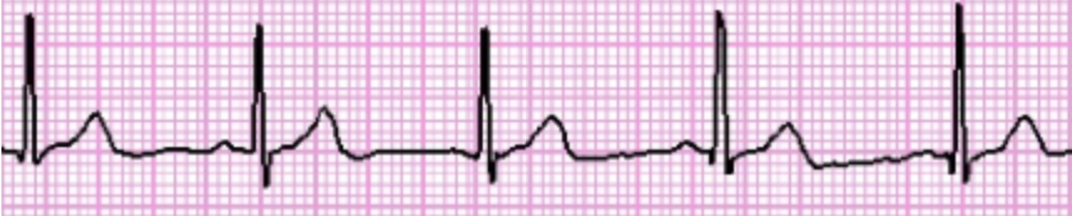
\includegraphics[width=100mm,scale=0.7]{ecgtrace}
	\caption{Example of ECG trace}
	\label{fig:ecgex}
\end{figure}

\subsection{Electrical Cell}
This cells have the exclusive capability to discharge electrical current without the necessity of external stimuli: this property is called automaticity , and the underlying mechanism is the sodium pump.\\In a resting cardiac cell the electrical charges are equally balanced and there is not electrical flow: the cell is said to be polarized or in the ready state.\\The automaticity property, allows this cell to modify the membrane and pull sodium inside and potassium outside, so that the resulting difference of potential causes an electrical flow: this is the basic sodium pump functionality that makes the cell in a state called depolarized or discharge state.\\Finally, after this step, the process to turn the depolarized state in the original restring one, is called repolarization and it consists of pulling out of the cell's membrane the  sodium and inside the potassium, bringing in the end the cell to the original resting state. The whole process is described in Fig. ~\ref{fig:ecgtrans}.  
\begin{figure}[H] \centering
	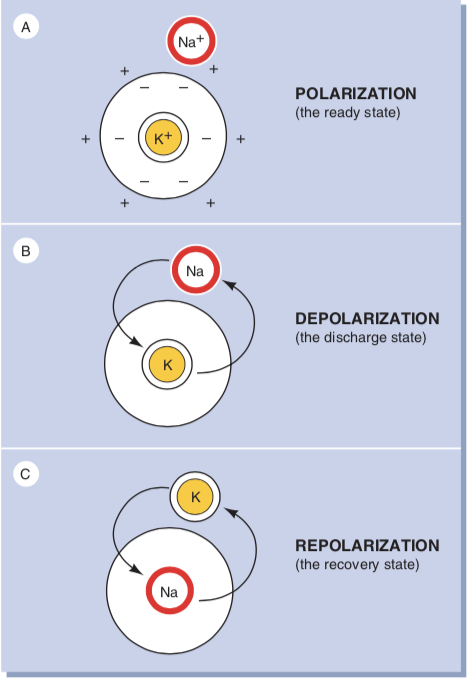
\includegraphics[width=80mm,scale=0.7]{ecgtrans}
	\caption{Electrical cell transactions: \cite{ecgbook}}
	\label{fig:ecgtrans}
\end{figure}
The heart is made of 4 chambers: two atriums in the upper part and two ventricles downside.The electrical cells conduct the current flow through a set of connections that overall constitute the conductive system and completely cover the heart's surface: this allows the consequent contraction of atriums and ventricles.
\subsection{Heartbeat Cycle}
Normally, the electrical impulse is produced in the sino atrial (SA) node positioned in the upper part of the right atrium.\\Then, it propagates down to the right atrium with the inter nodal pathways to reach the atrio ventricular node (AV) and left with  the inter atrial pathways to reach the left atrium. The entrance to the left and right ventricles is provided by the Bundle of His, through the left and right bundle branch, that terminates with Purkinje fibers who are in charge to contract the ventricles.\\It is interesting to note not all the portion of the heart have the same beat rhythm (beats per minute):
\begin{enumerate}
\item SA node: 60-100  
\item AV node: 40-60 
\item Ventricles: 20-40 
\end{enumerate}
The discussed structure is depicted in in Fig. ~\ref{fig:hearts}.
\begin{figure} \centering
	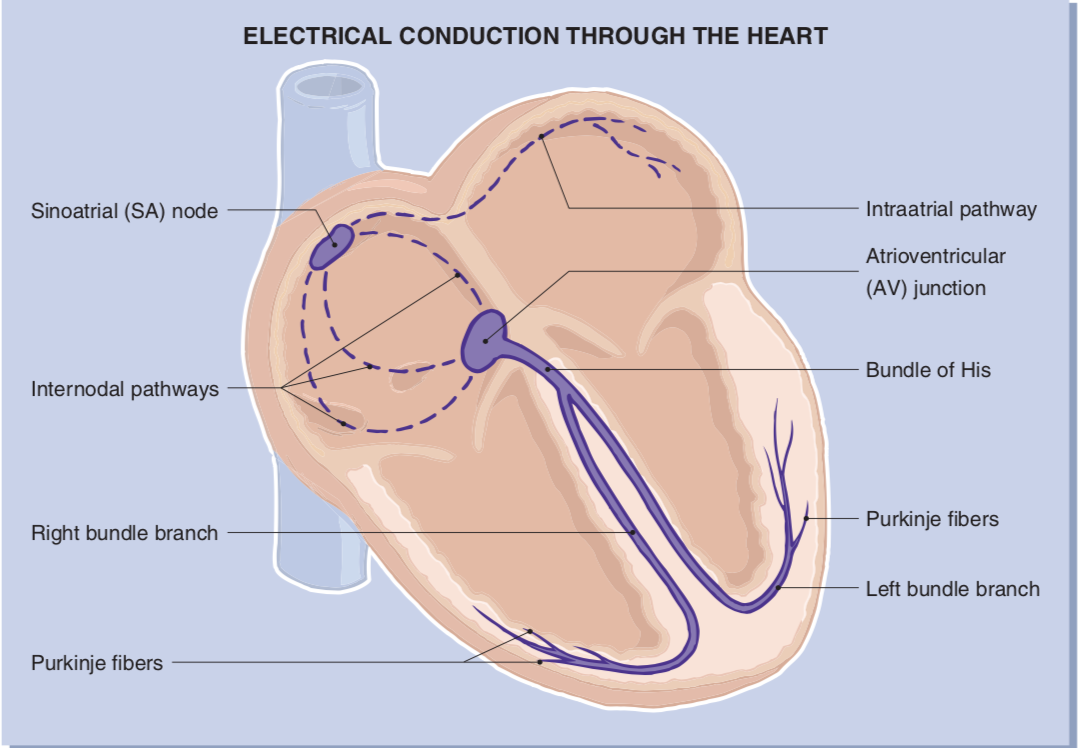
\includegraphics[width=100mm,scale=0.7]{heartex}
	\caption{Electrical tissue of heart: \cite{ecgbook}}
	\label{fig:hearts}
\end{figure}
In the ECG, in normal condition, the visible beat rate is due to SA node because it has the highest frequency and overrides all the other: this is the reason why it is defined as the pacemaker.\\The above values are called inherent rates and can help us to infer heart's dysfunctions visible in the ECG as a different SA rhythm. In a pathological context, for example if the SA node fails, the pacemaker becomes the AV node and  a slower rhythm is visible on the ECG: this callback safety mechanism is named escape.

\section{ECG tracing}
The acquired knowledge in the previous subsection, is essential to investigate how the electrical activity is transferred to graph paper to be analyzed for our task.\\The ECG is obtained placing some electrodes on the patient skin and connecting it, to a machine that will display the electrical activity.\\The location of the electrodes is crucial for the final output and it is possibile to obtain multiple views ( or lead) of the same heart, just by varying their position.\\In particular, some arrhythmias are more visible on a given view, and in general an effective diagnosis interpolate more leads. For example, in the dataset we consider, each ECG has two leads:
\begin{enumerate}
\item modified limb lead II (MLII) where the electrodes are on the chest.
\item modified chest lead V1 (MCL1) where negative electrode is placed close to the left shoulder and the positive electrode to the right of the sternum 
\end{enumerate}
For a long time, the most adopted lead has been the Lead II, and in the following I will take into consideration this configuration.\\However, there are different leads with better effectiveness.\\In Lead II the negative electrode is placed to the right, above the heart, while the positive to the left, behind the heart. In this way, when the electrical impulse propagates from the atrium to the ventricle, the ECG device will display an upright wave, while an upside down shape is generated in the opposite case (Fig. ~\ref{fig:ruleflow}).
Finally, the ECG is written on a conventional graph paper (Fig. ~\ref{fig:ecgex}) where the voltage levels are measured comparing the horizontal lines, and the time interval, considering the vertical lines: two consecutive vertical splits cover 0.04 seconds.
\begin{figure}[H]  \centering
	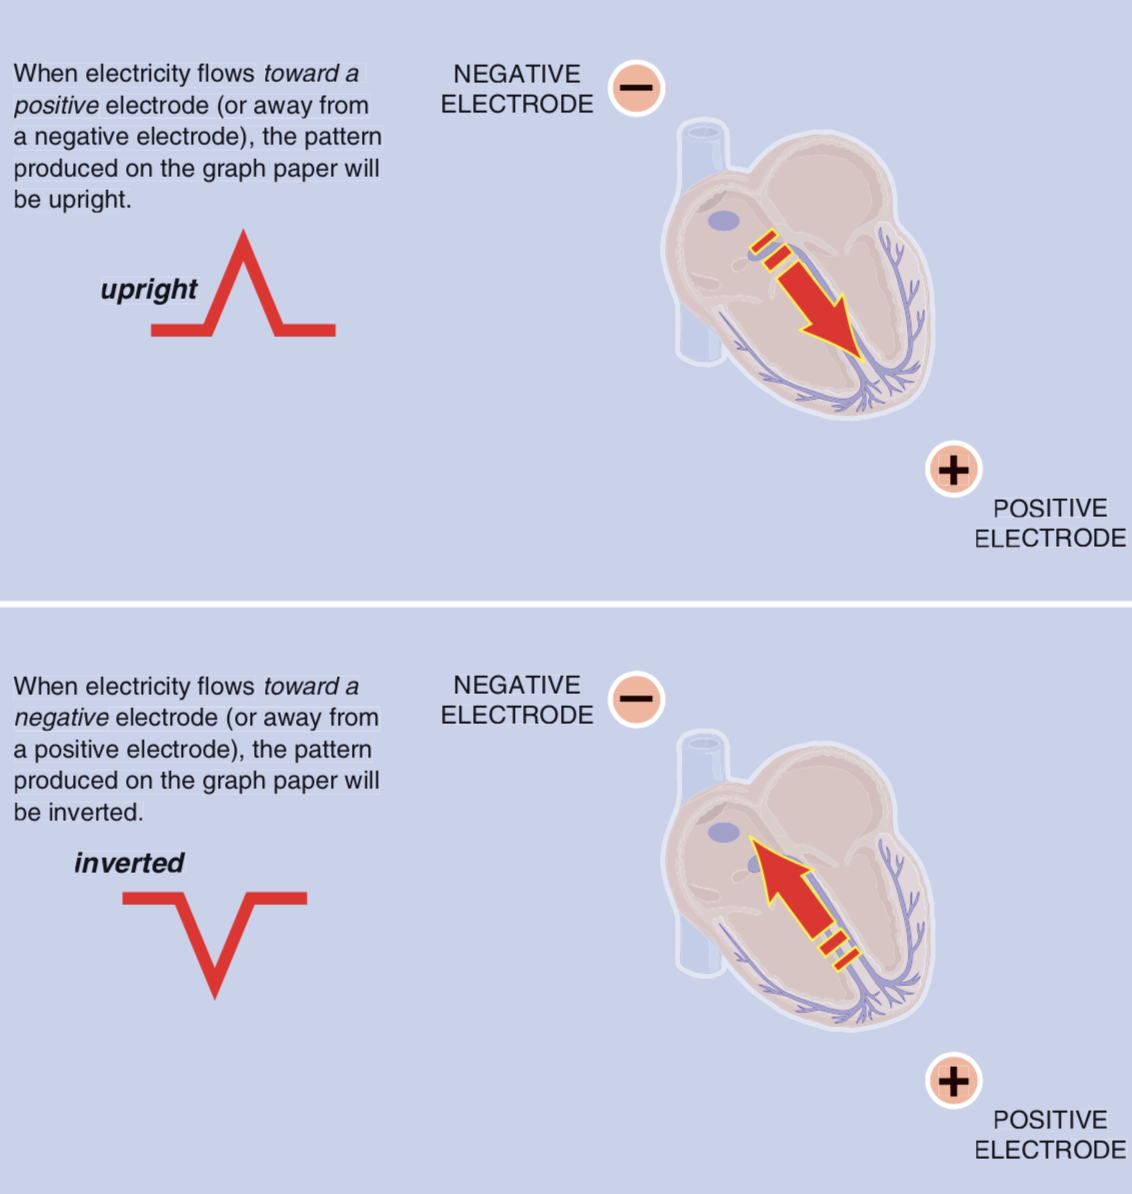
\includegraphics[width=100mm,scale=0.7]{ruleflow}
	\caption{Lead II basic principles: \cite{ecgbook}}
	\label{fig:ruleflow}
\end{figure}
\subsection{Heartbeat Shape}
During a normal beat, the heart first enter in the atria and then into the ventricles: this requires a synchronized mechanism so that while the atria fill, the ventricles contract and viceversa. During each phase of the cardiac cycle, a distinct pattern is produced on the ECG graph paper. This pattern describes instantly what is happening in the heart and it has the shape depicted in Fig. ~\ref{fig:beatshape}.
\begin{figure}[H]  \centering
	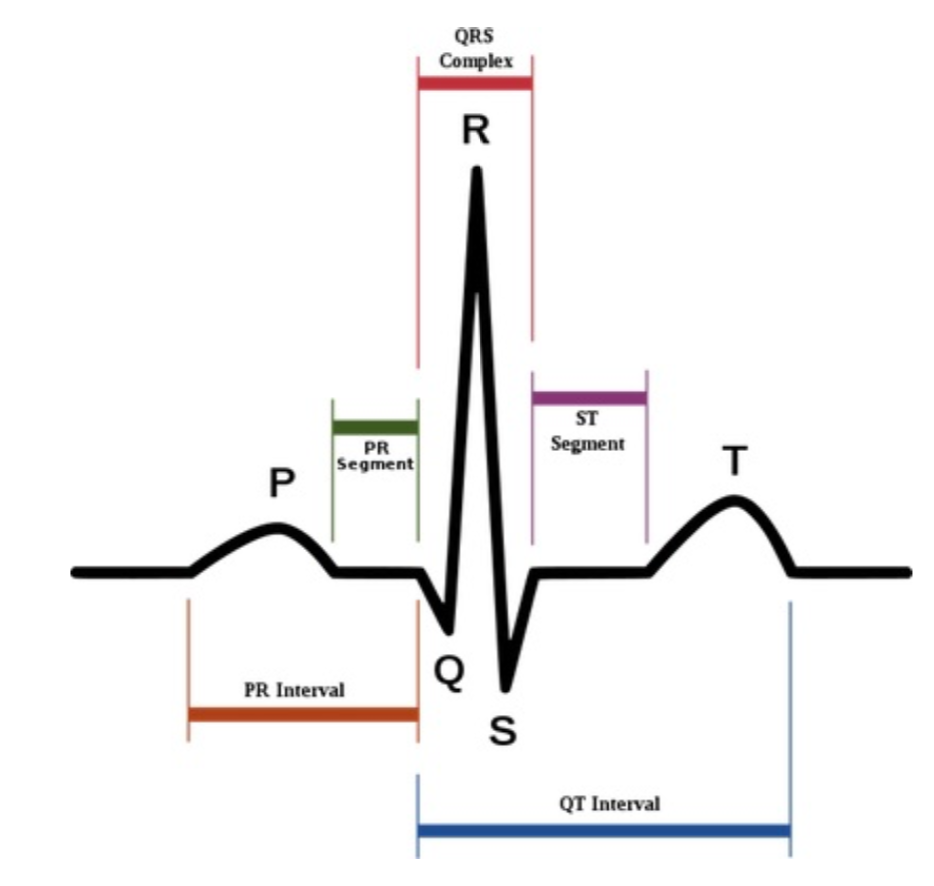
\includegraphics[width=80mm,scale=0.7]{beatshape}
	\caption{Heartbeat in the ECG}
	\label{fig:beatshape}
\end{figure}
The beat shape starts with a deflection: the P wave and it is generated by the SA node. Subsequently the impulse leaves the atria to reach the AV node and it encounters a slight delay because the encountered electrical tissues are slower. This is translated into a short period of electrical inactivity called the PR segment.\\The subsequent wave is the QRS complex, due to ventricular depolarization and it is significantly larger than the P wave because to  ventricles are greater than atria, so that more potential energy is required.\\The Q wave is defined as the first negative deflection following the P wave but before the R wave.\\This wave flows immediately into the R wave, which is the first positive deflection following the P wave. Next comes the S wave, which is defined as the second negative deflection following the P wave, or the first negative deflection following the R wave.\\After the ventricles depolarize, they begin their repolarization phase, which results in another wave in the ECG. The T wave is indicative of ventricular repolarization.\\The atria also repolarizes, but this event is not significant enough to show up in the ECG.\\Between the S and the T wave is a section called the ST segment.\\The ST segment is the flat, isoelectric section of the ECG between the end of the S wave and the beginning of the T wave. It represents the interval between ventricular depolarization and repolarization, and anomalies in this segment are symptom of infarction.

\subsection{Type of Arrhythmias}
Arrhythmia analysis is a complex task due to the high variability of the heart's mechanism inside each patient. Arrhythmias are classified into two classes:
\begin{enumerate}
\item rhythmic: constituted of a series of irregular beats
\item morphological: single abnormal beat
\end{enumerate}
This work is concentrated on the latter.\\Morphological arrhythmias are classified into 4 macro classes by the Association for the Advancement of Medical Instrumentation (AAMI) standard, with respect to the location where the anomaly starts:
\begin{enumerate}
\item N-class. It happens when the beat regularly starts at the SA node but can be blocked in the left or right bundle branch.It includes regular beat.For example, left bundle brach block, happens when the impulse does not reach the left ventricle because the left bundle is compromised: in this situation , first the right ventricle will depolarize and then also the left one. This results in a QRS complex longer than 120 ms.
\item S-class. It happens when the impulse starts below the SA node: in this situation the impulse will begin at the bottom and subsequently will reach the upper part, resulting in an upside down P wave.
\item V-class. It happens when the impulse originates in the ventricles and it shows up in the ECG as a tall and wide QRS
\item F-class. It happens when there are multiple sources of depolarization: for example in Fig. ~\ref{fig:arrhex} the P wave is modified by an additional source of depolarization
\end{enumerate}
\begin{figure}[H]  \centering
	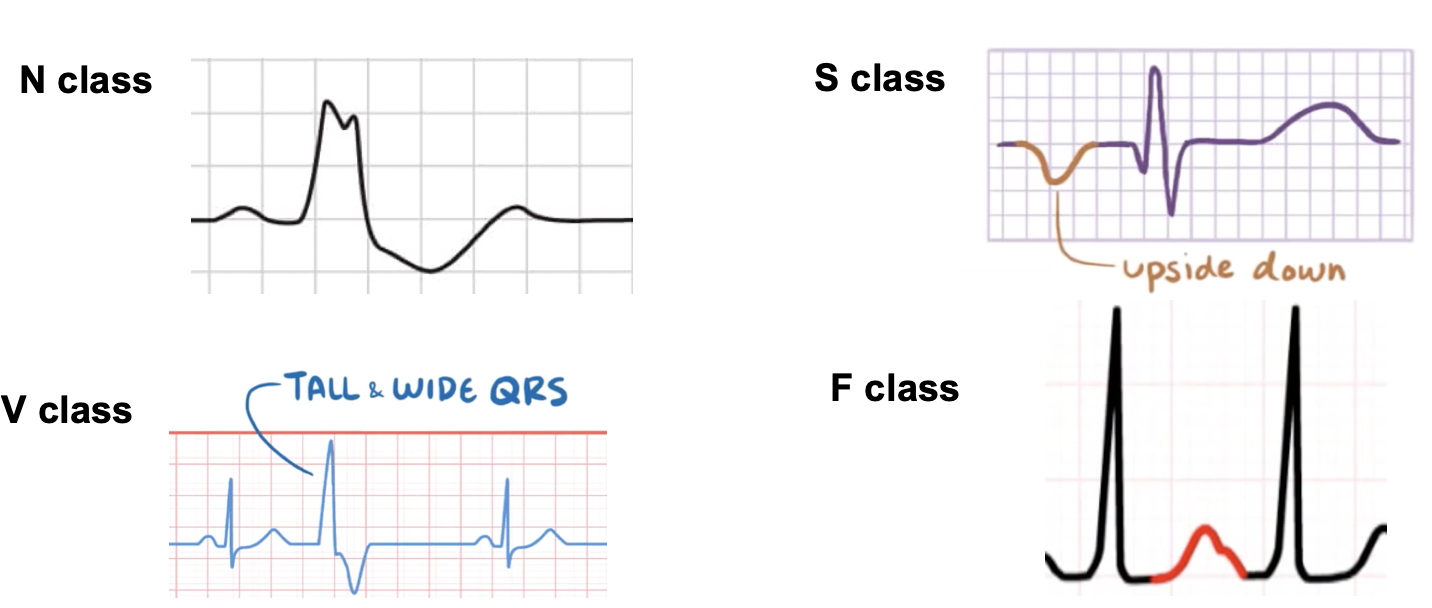
\includegraphics[width=100mm,scale=0.7]{arrhex}
	\caption{Examples of Arrhytmias}
	\label{fig:arrhex}
\end{figure}
A more detailed arrangement of the above classes are depicted in the figure below.
\begin{figure}[H]  \centering
	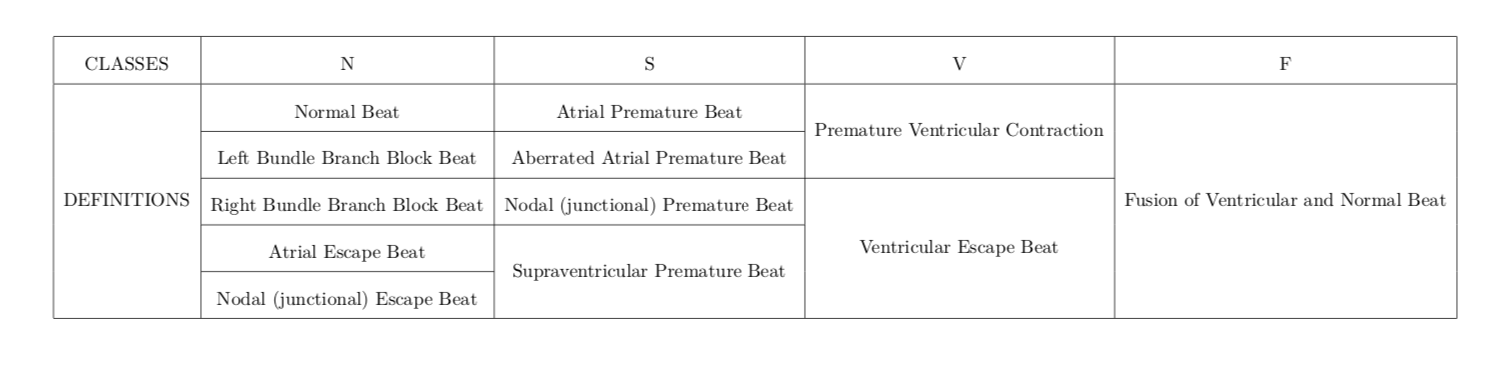
\includegraphics[width=150mm,scale=0.7]{allclass}
	\caption{Detailed classification of arrhythmias }
	\label{fig:allclass}
\end{figure}

\chapter{Pre-Processing}
As we have previously, discussed, the ECG tracing is an empirical process prone to noise measurements whose removal is of high importance to guarantee the detection of the relevant features without incurring into overfitting issues.\\The principal methods to remove noise are based on frequencies domain analysis : in the following I will describe Median Filter and Discrete Wavelet Transform.\\In addition to this, the dataset we are taking into consideration is highly over balanced: one class constitutes more than 80\% of all the elements: this can lead to inconsistencies because an algorithm could reach high accuracy, merely predicting only that class without any generalization competence.\\For the purpose of handling the latter, we have used several approaches based on data augmentation and weighted loss function. 
\section{De-Noise}
The ECG  can be affected by several sources of noise during the recording, attributable to : 
\begin{enumerate}
\item Baseline wander caused by patient's movements.It is visible in the signal with frequencies below 0.5 Hz (Fig. ~\ref{fig:n1}.a ).
\item Power line interference caused by electromagnetic external devices.It appears in the signal as 50/60 Hz sinusoids (Fig. ~\ref{fig:n1}.b ) .
\item Muscle artifact caused by muscle activity near the electrode for the contraction of the heart's patient. It is difficult to be removed since it is strictly related with the electrical impulse of the ventricles that determines the QRS complex on the ECG. Its removal can result in unwanted distortion of the signal (Fig. ~\ref{fig:n1}.c ) .
\end{enumerate}
\begin{figure}[H]  \centering
	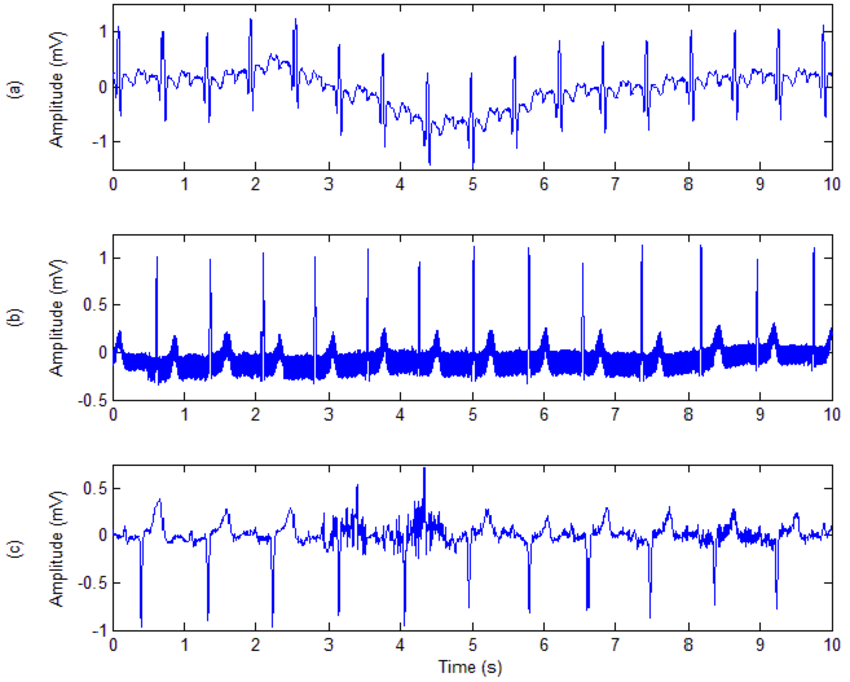
\includegraphics[width=100mm,scale=0.7]{noise.png}
	\caption{Example of noise in ECG recordings. (a) Baseline wander, (b) Power line interference, and (c) Muscle artifact. \cite{noise}}
	\label{fig:n1}
\end{figure}
It is crucial to note the role of de-noise algorithms is to clean the signals without loosing relevant information:  after the processing, the filtered signal must contain the original key features of a beat in terms of P,Q,R,S,T wave.\\In this project we have considered 2 different ways of noise removal : median filter and discrete wavelet transform (DWT).

\subsection{Median Filter}
A median filter takes as input a signal $S = [x_1 , \dots , x_n]$ and a window of size : $w$.\\It returns a converted signal where for every sample : $x_i \in S$, it is computed the median of the elements : $[x_i, x_{i+1}, \dots , x_{(i+w) \; mod \; n}]$.\\The intuition behind a median filter, is that noisy samples tends to have too high or too low values, with respect to the neighbor samples : replacing them with the median in a given range can be a good approach.\\This technique is used in \cite{rfdwt} to mitigate the noise due to baseline wonder.




\subsection{Discrete Wavelet Transform}
The ECG signal is non stationary because beats are generated by the heart under influences of physiological factors that depend on the brain and change continuously over the time.\\In order to characterize it, a simple approach could consist of a time domain analysis, taking into consideration factors like the duration of QRS complex or ST segment.\\However, this approach does not fit with the subtle changes in the amplitude and duration in the ECG that are specific for any patient.\\Another approach is to perform a frequency domain analysis with Fourier Transform.\\However, the latter is not perfectly applicable because it is not accurate to assume that a given frequency is equally distributed in the signal: this is only true for periodic, stationary signal.\\In particular, to represent the ECG signal we are interested not only in the frequency contained, but also in the portion of the signal exhibits a given frequency.\\With the aim of having a better resolution in time, it is possible to study the frequencies of the signal present in a temporal window of the signal: for example we can study the frequencies of the signal from $t=0$ to $t=0.1$, so that we can infer the frequencies localized in the interval.\\However, the drawback of this approach is that it is not possible to detect all the frequencies because in that window we can only find the frequencies greater than $\frac{1}{0.1}=10 Hz$ , since for frequencies greater than $10 Hz$ we need to consider a widow larger than: $0.1s$.\\The explained tradeoff between frequency and time resolution is the application of the Heisenberg's Uncertainty Principle.\\In order to mitigate this issues: the optimum approach is to consider small window for high frequencies and large window for low frequencies.\\In fact, when a signal component is rapidly changing it is essential to detect the instant when this happens.\\on the contrary, when a component repeats slowly it is necessarily a larger window to detect it.\\The Discrete Wavelet Transform (DWT) takes advantage of this latter consideration.\\DWT considers as basis function a wavelet instead of sinusoid employed by Fourier Transform.\\A wavelet is a function with with a limited duration : it has an amplitude that begins at zero, increases, and then decreases back to zero. A wavelet is more localized in time than a sinusoid because it exists only in a restricted interval (Fig. ~\ref{fig:we} ). 
\begin{figure}[H]  \centering
	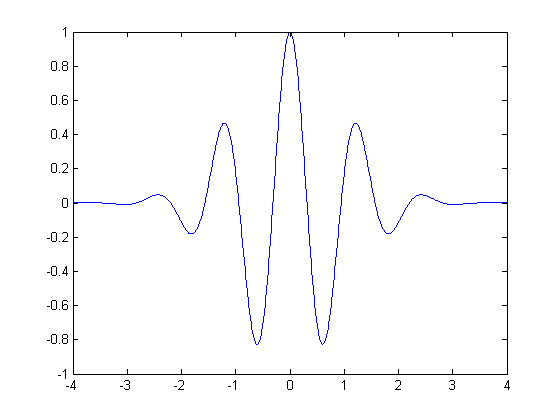
\includegraphics[width=80mm,scale=0.7]{waveletexample.png}
	\caption{Wavelet named Meyer}
	\label{fig:we}
\end{figure}
The main parameters of a wavelet are:
\begin{enumerate}
\item scaling.The scale of a wavelet is a measure of how it is expanded, so that the higher the scale the more it is spread and the less it is localized in time (Fig. ~\ref{fig:ws} ).
\item shifting.The wavelet is shifted across the input signal to align it with the features we are interested in, for example the QRS complex.
\end{enumerate}
\begin{figure}[H]  \centering
	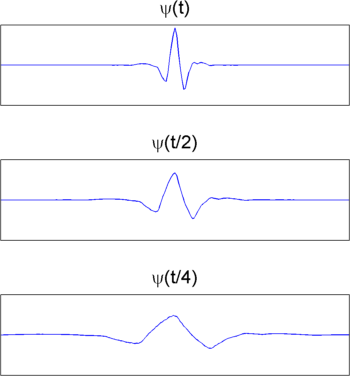
\includegraphics[width=80mm,scale=0.7]{wavescale.png}
	\caption{Wavelet with scaling factor of 1,2,4: \cite{matdwt} }
	\label{fig:ws}
\end{figure}
In general the idea of DWT is to analyze the correlation between the signal and a given wavelet shifted over the signal with increasing scale: initially it is analyzed high frequency behavior and at each successive step the scale is doubled and the signal downsampled for the Nyquist criterion.\\In conclusion, DWT outputs the signal at different bandwidth, such that at each level of analysis, the output is high, if there is a strong correlation of the signal at that frequency with the wavelet at that scale.\\There are several families of wavelet, and the choice of the correct one, relies on the similarity of shape with the portion of ECG we are interested (Fig. ~\ref{fig:wf}) .\\For example, a common choice is the Meyer wavelet (Fig. ~\ref{fig:we} ) because it is comparable to the QRS complex.\\DWT is mainly used as :
\begin{enumerate}
\item a filter ignoring the coefficients at a given frequency level while reconstructing the signal (\cite{lnlf}).
\item feature selection considering the coefficients with high value, or with high correlation with the original signal (\cite{rfdwt},\cite{lnlf}).
\end{enumerate}
\begin{figure}[H]  \centering
	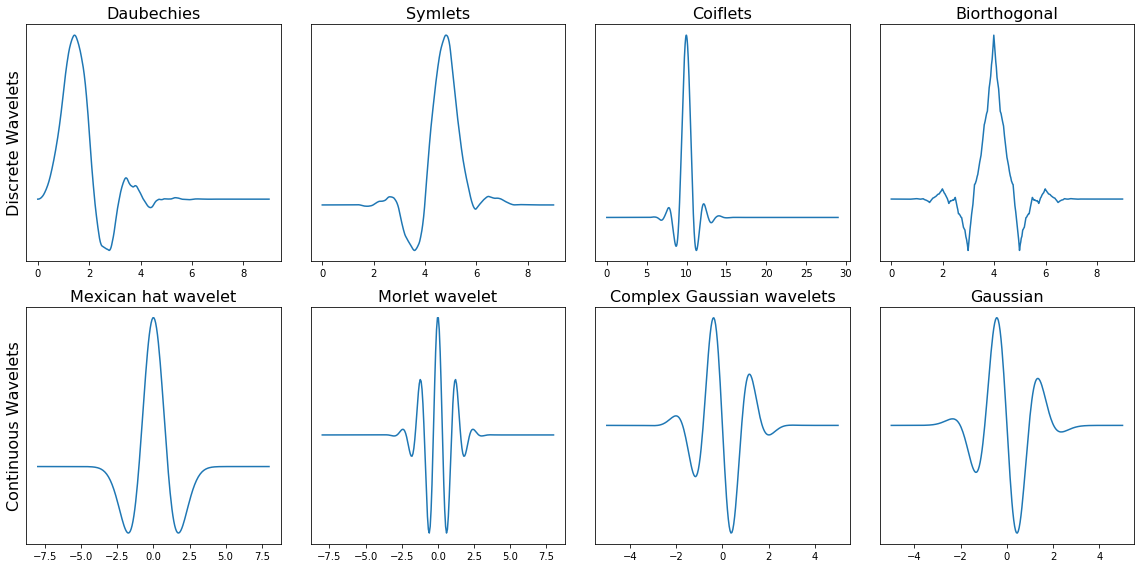
\includegraphics[width=100mm,scale=0.7]{waveletfamilies.png}
	\caption{Wavelet families: \cite{watut} }
	\label{fig:wf}
\end{figure}





\section{Data Augmentation}
The dataset's details will be discussed later: so far it is important to note it is overbalanced. In particular the N class is more than 80\% of the whole dataset.\\Models trained on imbalanced dataset do not acquire any generalization power: they are biased toward the most populated class and fail to detect the distinguish features of the others.\\For example in our case, a model could reach a high accuracy during the train just by learning to always predict the same class.\\Class imbalance is typical of biological dataset, where the interest is towards minority samples that are linked to rare events (\cite{conf/ijcnn/HeBGL08}).\\We have tried to solve this issue using the following methods: Smote, Adasyn and weighted loss function for neural networks.\\In the following, I will use the following notation:
\begin{enumerate}
\item Dataset: $D$, with $n$ samples: $D=\{(x_1,y_1),\dots,(x_n,y_n)\}$
\item Classes: $Y=\{1,-1\}$ such that $|y_i \in Y$. For now we consider only two classes, but the same considerations can be generalize to $N$ classes 
\item $m_s$ and $m_l$ is the number of samples belonging respectively to the under-balanced and over-balanced class: $m_s\leq m_l$ and $m_s+m_l=m$
\end{enumerate}
\subsection{Smote and Adasyn}
In order to build a consistent dataset, it is possible to add new elements to the less populated class (over-sampling), or to remove existing samples of the most populated class (under-sampling). We have adopted the first one, 
to take advantage of all the information contained in the dataset even for unbalanced classes. The main oversampling algorithms are Smote (\cite{smotepaper}) and Adasyn (\cite{conf/ijcnn/HeBGL08}). The latter is an improved version of the first one. \\In general, Smote takes into consideration a given class and generates $N$ additional synthetic examples for each original element. For example, if $N$ is 1, the size of the class is doubled.\\Specifically, this algorithm performs the following steps:
\begin{enumerate}
\item take a sample: $x_i$, and consider the difference vectors $z_1,\dots,z_n$ between $x_i$ and the $K$ closest neighbors of the same class: ${x_j,\dots,x_{j+K}}$. In the end, $z_j = x_i - x_j$  where $1\leq j,i\leq n$
\item for every $N\leq K$, randomly chosen, difference vectors: $z_j$, returns a new sample: $s_j = x_i+r\cdot d_j$ where $r \in [0,1]$ is a random value.
\end{enumerate}
In the end, a new point is a randomly positioned in the segment whose extremities are the original sample and its neighbor.This approach effectively forces the decision region of the minority class to become more general (\cite{smotepaper}). However, Smote does not create representative samples when the under-balanced class has extreme values: in this case the created element will be centered in the dataset space even if the under-balanced samples will probably lie on the boundary.
\begin{figure}[H]  \centering
	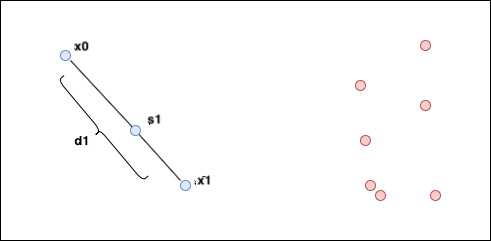
\includegraphics[width=80mm,scale=0.7]{smoteex.png}
	\caption{The blue class is underbalanced: Smote generates a new sample: $s_1$ between $x_0$ and $x_1$}
	\label{fig:smoteex}
\end{figure}
Adasyn is an advanced version of Smote: the main difference is the first automatically detect the number of samples to generate: $g_i$, with respect to the element considered in the under-balanced class: $x_i$.In general, more samples will be created for samples whose neighbors belong to another class. The idea is that missing points should concentrate in the dataset space where a given element is under-represented.\\Specifically, it performs the following steps:
\begin{enumerate}
\item $d = \frac{m_s}{m_l} \in [0,1]$ is a measurement of class imbalance. We define a threshold value: $d_{th}$ as limit to the maximum class unbalance: if $d_i\le d_{th}$ the algorithm terminates.
\item $G=(m_l - m_s)\cdot \beta$, where $\beta \in [0,1]$. $G$ is the total number of new samples to generate. $\beta$ is user defined, for example if $\beta=1$, the resulting dataset is completely balanced.
\item $r_i = \frac{\Delta_i}{K} \; i \in \{1,\dots,m_{s}\}$, where:
\begin{enumerate}
\item  $\Delta_i$ is the number of the $K$ closest neighbors to $x_i$, belonging to the other class: this is different from Smote where we consider only the samples of the same class as neighbors
\item $r_i \in [0,1]$ and it indicates how $x_i$ is isolated from the rest of points belonging to the same class
\end{enumerate}
\item $0\leq \hat{r_i}=\frac{r_i}{\sum_{i=0}^{m_s}r_i }\leq 1$. In this way, $r_i$ is normalized: $\sum_{i=0}^{m_s}\hat{r_i} =1$
\item $g_i=\hat{r_i}\cdot G$. It is the number of samples to generate for each minority sample: $\sum_{i=0}^{m_s}g_i =G$ 
\item for each minority sample creates $g_i$ samples $s_j$, in the same way of Smote: $s_j = x_i+r\cdot d_j$
\end{enumerate}
The idea is that $\hat{r_i}$ measures how difficult it is, to learn the features of $x_i$: greater values of $r_i$ are indicative that $x_i$ is an outlier and hard to generalize it: the more a sample is difficult to learn, the more Adasyn will generate new elements related to it. Finally, it is possible to generalize Adasyn to the multi-class case just by varying the value of $\Delta_i$: it can be computed as the number the samples belonging to the most populated class or to any different class.



% le ho usate poco solamente per replicare un paper
%\chapter{Feature Extraction}
%A crucial issue is the choice of the number of samples that make a beat and the features that characterized it.\\The %main techniques used to obtain representative features are DWT (again), principal component analysis (PCA), %independent component analysis (ICA), high order statistics (HOS).
%\section{Principal Component Analysis }
%VEDI PAPER LINEAR NOT LINEAR
%\section{Independent Component Analysis }
%VEDI PAPER LINEAR NOT LINEAR
%\section{High Order Statistics }
%VEDI PAPER LINEAR NOT LINEAR
%

\chapter{Classification Algorithms}
The algorithms used for the final classification are: Random Forest, Support Vector Machine and Neural Network.
\section{Random Forest}
\section{Support Vector Machine}
\section{Feed Forward Neural Network}
\subsection{Activation Function}
\subsection{Loss Function}


\section{Convolutional Neural Network}
Convolutional Neural Networks (CNN) are a deep models that performs well with a variety of tasks such as image classification, natural language processing and signal processing. CNNs are explicitly designed to deal with multi dimensional input and overcome the high number of parameters that is requested by standard FNN. For example a single RGB image of size 64x64, in a FNN would require: $64\cdot64\cdot3=12288$ neurons as input.\\The issues that arise when the FNN is over parametrized are the following:
\begin{enumerate}
\item a huge number of input neurons, will require more layers at a high computation cost and time required for training 
\item over-parametrization is symptom of overfitting: in the specific case of an image, the FNN would behave too meticulous since it will take into account each single pixel
\end{enumerate}
In order to take into account the multidimensional input, CNN's neurons are organized in three dimensions and to reduce the overall complexity, the neurons in each layer are connected only to a portion of the previous one. This is the opposite of what happens in fully connected neural networks. 
\begin{figure}[H]  \centering
	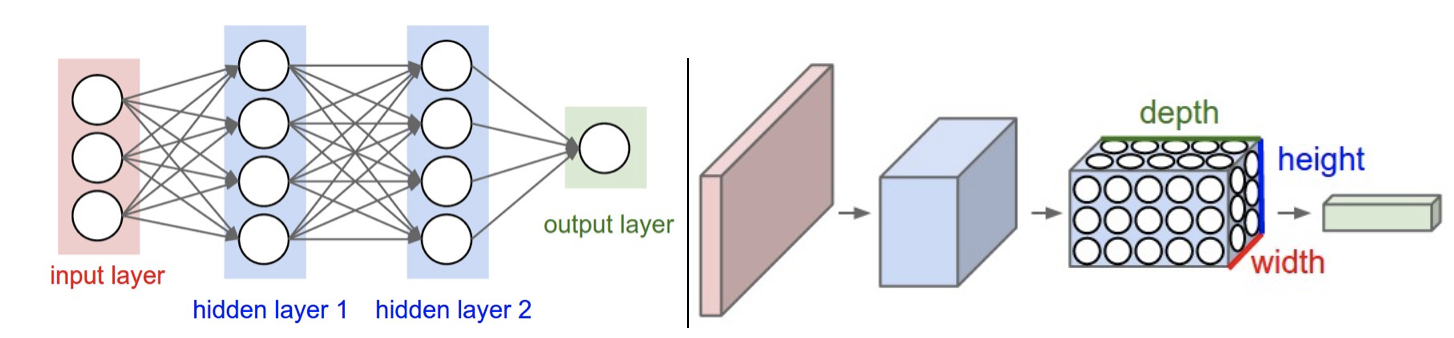
\includegraphics[width=150mm,scale=0.7]{convgen}
	\caption{Comparison of FNN versus CNN. In CNN each layer has 3 dimension: depth, height, length.\cite{cnnsite}}
	\label{fig:convgen}
\end{figure}
The main types of layers used in a CNN are:
\begin{enumerate}
\item convolutional: consists of groups of neurons apply scalar product with the connected portions of the input.
\item pooling: downsampling to reduce the dimensionally 
\item fully connected: produces the final predictions. Generally, it is preceded by a flattening operation since the convolutional outputs are always 3 dimensional
\end{enumerate}
\subsection{Convolutional Layer}
The convolutional layer is the building block of CNNs. It consists of a set of filters (or kernel), whose parameters are learnt during the training.\\A single filter is a multidimensional matrix with a height, length and same width of the input layer. For example if we have an RGB image of size: $64\cdot64\cdot3$ and filer of size: $6x6x3$, the total number of learnable parameters of the latter are: $6\cdot6\cdot3=108$. It is immediate to note the crucial reduction of parameters with respect to a classical feed forward neural network, that wold have required $64\cdot64\cdot 3=12288$ weights in the input layer.\\During forward pass, each filter is shifted through the input and performs a convolution that in practice is a simple dot product.\\The filter can be interpreted as a particular feature and the convolution asses how much that feature is present in the portion of input. During the training, the CNN learns the weights of such filters, so that they can extract the actual features to discriminate the final prediction. In the end, each filter outputs a 2 dimensional matrix that for what we said before it is called feature map.\\As we said before, each filter has a limited area called receptive field that is connected only to a small portion of the input to reduce the number of parameters.\\This technique as the name suggest is called parameter sharing and is based on the fact the same feature is present in multiple region of the input: for example if we want to detect the border of an image, we could use a filter that properly activates when it is convoluted with them. In any case, the filter is applied to all the input and at the end of any convolutional  layer is always present an activation function that is generally a ReLU.
\begin{figure}[H]  \centering
	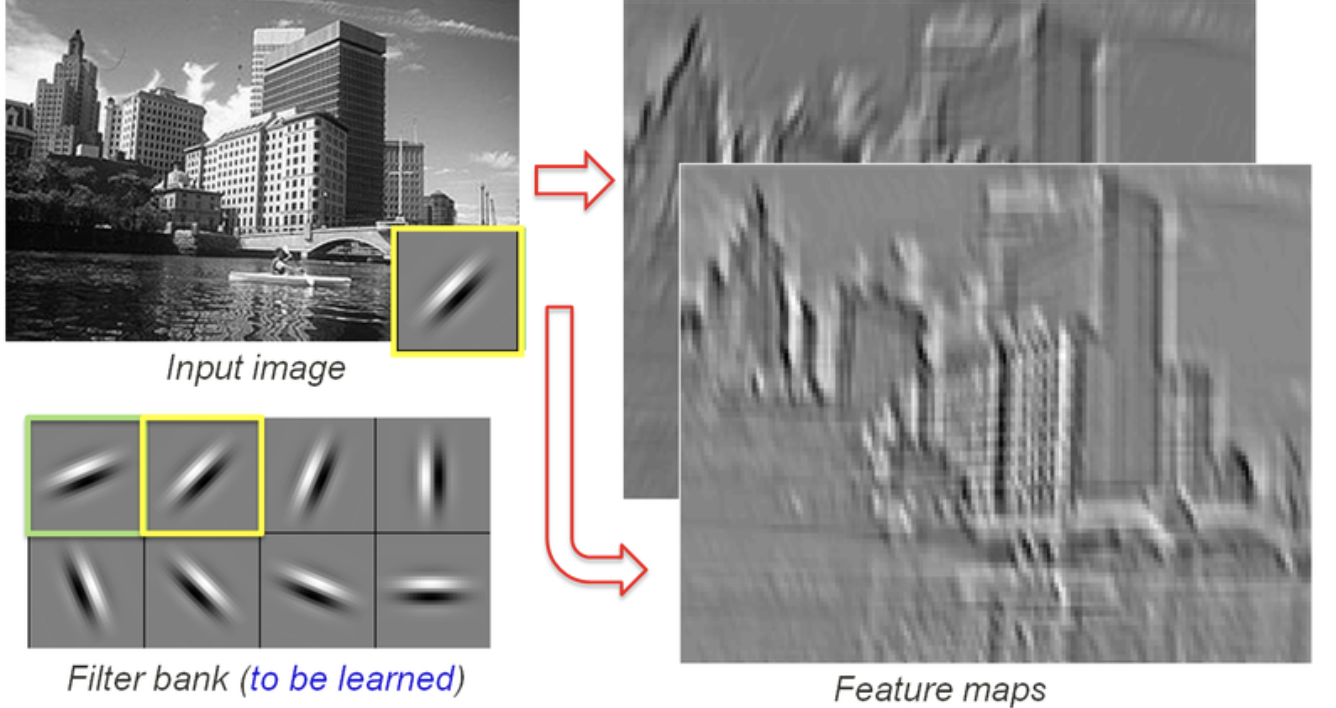
\includegraphics[width=80mm,scale=0.7]{exfilter}
	\caption{2 different filters are applied to the input image, resulting in 2 different feature maps \cite{cnnstackoverflow}}
	\label{fig:exfilter}
\end{figure}
The parameters of a convolutional layer are:
\begin{enumerate}
\item spatial extent of the filter ($F$)
\item depth ($K$): the number of filters that determines the depth of the output
\item stride ($S$): the number of pixels to skip every time the filter is convoluted
\item zero-padding: consists of adding some zeros to the image border to have control on the output dimension. Specifically if $P=1$ each border has one zero and so on.
\end{enumerate}
With the notation above, we can deduct the output dimension of a convolutional layer. Given an image of size: $W_1 \cdot H_1 \cdot D_1$, the output is:
\begin{enumerate}
\item $W_2 = 1+(W_1-F-2P)/S$
\item $H_2 = 1+(H_1-F-2P)/S$
\item $D_2 = K$
\end{enumerate} 
The number of parameters for a single filter are: $F\cdot F\cdot D_1$ and globally: $F\cdot F\cdot D_1\cdot K$
\subsection{Pooling Layer}
The pooling layer is used to reduce the dimensionality of the given output's layer and consequently to obtain a reduced number of parameters at a less computational cost.\\Generally, it has a local extension of 2x2 ($F=2$) and it outputs the maximum in the region it is applied (max pooling) with a given stride: $S$. It performs a downsampling only through the width and height: the original depth is left unchanged.\\Also in this case it is possible to define the output dimension as:
\begin{enumerate}
\item $W_2 = 1+(W_1-F)/S$
\item $H_2 = 1+(H_1-F)/S$
\item $D_2 = D_1$
\end{enumerate} 
\begin{figure}[H]  \centering
	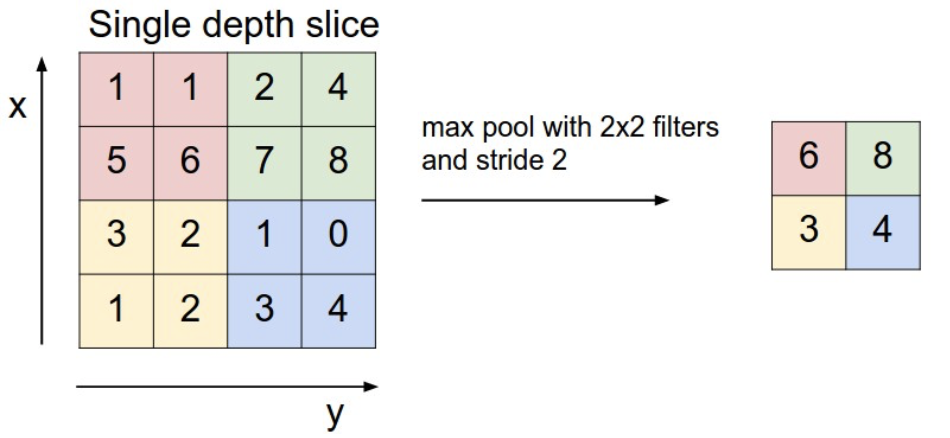
\includegraphics[width=80mm,scale=0.7]{pool}
	\caption{Max pool with stride 2.(Left: original input, Right: pooling output) \cite{cnnsite}}
	\label{fig:pool}
\end{figure}

\subsection{Mathematical Interpretation}
In this section, I will describe CNNs from a geometric point of view, so that it is possible to understand the necessity of an activation function at the end of each layer and the advantages of multiple stacked convolutional layers.\\In \cite{cnninter}, the CNN is interpreted as a RECOS model: set of operation that performs Rectified Operation On a Spere. Specifically, each filter is interpreted as an anchor vector in a sphere, because they serve as reference signals.\\Each convolution between a local region and filter, is translated as a similarity score between the anchor vector and the vector representation of that region.\\In the RECOS model, negative correlation are set to zero, and the reason will be described later.\\Given a image's region in a vectorial form: $x=(x_1,\dots,x_N)^T$, and a sphere centered in the origin of unitary size: $S=\{\boldsymbol{x}\mid ||x||=1\}$, we analyze the geodesic distance between $x$ and an anchor vector: $\boldsymbol{a_1}$.\\In particular, the geodesic similarity: $d$ is the output of the convolutional step between a filter and the portion of input it is applied, that is a simple dot product.\\Specifically, $d=\boldsymbol{a_1}^T \boldsymbol{x}=cos(\theta)$ where $\theta$ is the angle between the two vectors (Fig. ~\ref{fig:geocnn}). The longer the correlation, the shorter the distance.
\begin{figure}[H]  \centering
	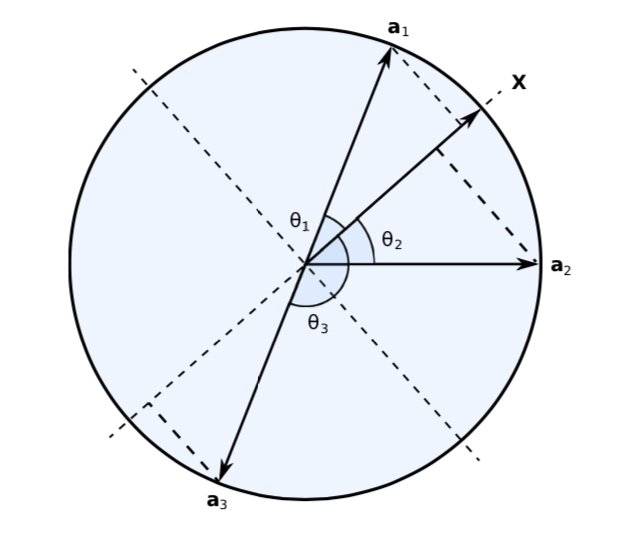
\includegraphics[width=70mm,scale=0.7]{geocnn}
	\caption{An input vector $\boldsymbol{x}$ with three anchor vectors: $\boldsymbol{a_1,a_2,a_3}$, in the sphere S: \cite{cnninter}}
	\label{fig:geocnn}
\end{figure}
The problems with this similarity score, happen when $\theta>90$, because $cos(\theta)<0$. Even if we could state a negative value correctly indicates high distances, issues arise when an additional anchor vector is negatively convoluted on the previous output producing a positive outcome. In this case, low correlated anchor vectors have outputted a positive score.\\Similarly, the model is not able to distinguish with two anchor vectors, between positive/negative response and viceversa.\\To solve this problems, we apply a Rectified Linear Unit (ReLU) so that negative correlation are set unambiguously to zero.\\The paper (\cite{cnninter}), further discuss the need to multiple convolutional layers.\\The point is that each layer operates at different pattern level detection: from more general to more specific patterns.\\For example, the paper tested on MNIST dataset that by changing the background's images, the first layer's filters change while the second layer is unaltered.\\This is due to the first layer is more general and capture the general picture so also the background, while the following ones tends to concentrare on more specific invariant features.\\Finally, I will conclude with the role of the fully connected layers.\\Generally, the convolutional layers perform feature selection, while the last dense layers are used to detect the surface boundary required for the final classification.\\In details, the latter need to cluster the input vector  to the specified dimension. For example with a FC layer of size 100 and 4, the features are first clustered to 100 clusters and then to 4.

\section{Recurrent Neural Network}
Recurrent Neural Networks (RNN) have been introduced in 80's for modeling time series, because traditional approaches based on FNN were not appropriate. The latter operate under the assumption each element of the input data is independent from the others. Since the information only flows in the forward direction in every layer of the network, it does not take into account the information contained in the order of the input.\\However, the order is crucial for tasks such as time series regression, word sense disambiguation and in general any problem where the input is an ordered sequence.\\For example, if we want to predict the Amazon's stock price in August 2019, we need to take into consideration the sequence of stock prices in July,June and so on: temporal dependency (Fig. ~\ref{fig:amzsp}).
\begin{figure}[H]  \centering
	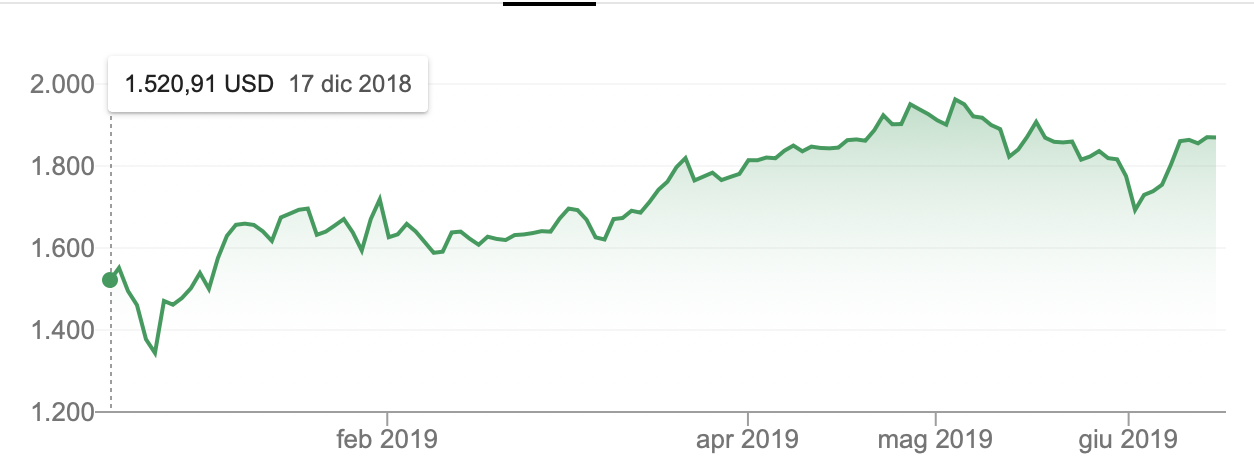
\includegraphics[width=100mm,scale=0.7]{amzsp}
	\caption{Amazon stock price in 6 months. To predict its value in August, the RNN could consider the fact in June has a positive and the same could happen in August}
	\label{fig:amzsp}
\end{figure}

If we need to disambiguate the sense of a word, it is necessarily to evaluate the position of that word in the phrase: spatial dependency. In the specific case of arrhythmia detection, it is required to capture the spatial dependency among samples, to detect features like the QRS complex, ST segment.\\The same dependencies the RNN aims to capture, characterize also the human learning process. As human being we learn the sequence not the symbols alone: for us it is immediate to say the alphabet from A to Z, but in the opposite direction is not straight forward. The same is true for our telephone's number. In order to model dependencies, RNN has an internal memory that is continuously updated through the input sequence.\\ In the following I will first describe Vanilla RNN, the vanishing gradient problem and how LSTM solves the latter.

\subsection{Vanilla RNN}
The intuition to make explicit the sequence dependency in a RNN is to feed each layer with the previous one through a retroactive loop (Fig. ~\ref{fig:rnnmod}).
\begin{figure}[H]  \centering
	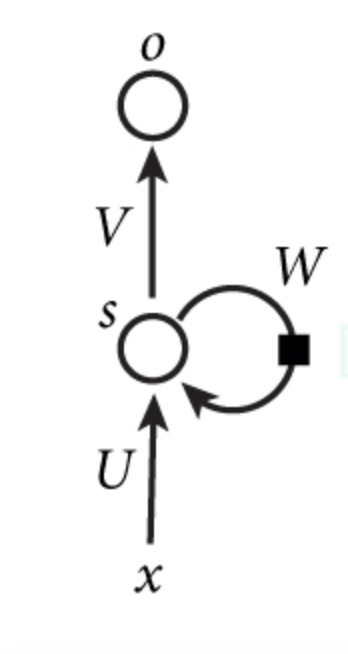
\includegraphics[width=30mm,scale=0.3]{rnnmod}
	\caption{RNN general structure \cite{recsite}}
	\label{fig:rnnmod}
\end{figure}
In this way, a sample $x_t \in S=[x_1,\dots,x_T]$, is fed into the RNN to produce the output $o$ and a hidden state: $s_t$ that will be taken into consideration by the network for the next sample: $x_{t+1}$.\\This structure can be unrolled in multiple blocks so that the loop is deleted, as shown in Fig. ~\ref{fig:unrolled}: in this way it is clear how the output $o_t$ depends on the current input: $x_t$ and previous state: $s_{t-1}$
\begin{figure}[H]  \centering
	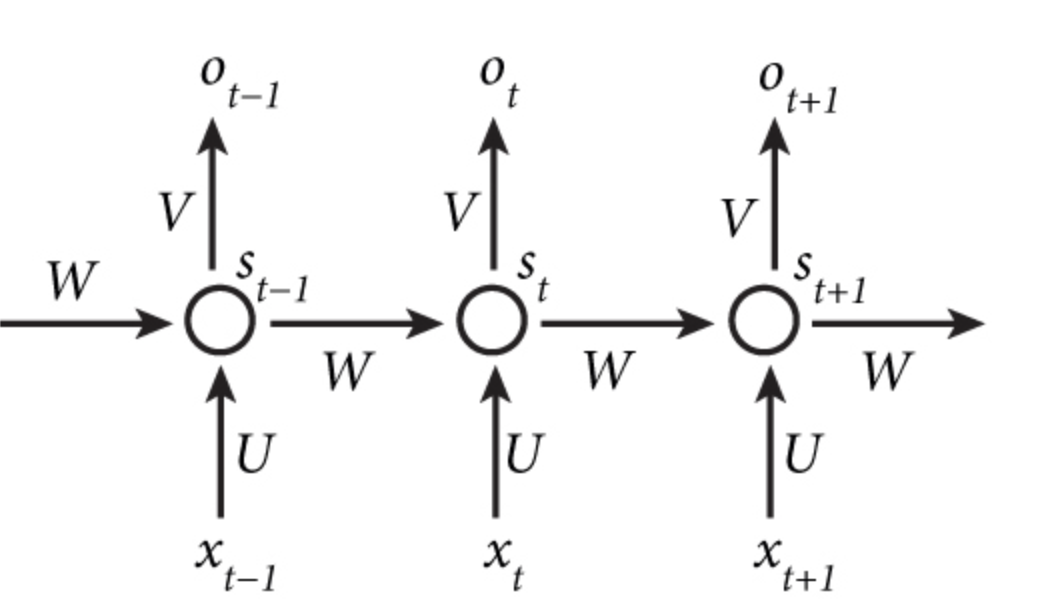
\includegraphics[width=80mm,scale=0.7]{unrolled}
	\caption{RNN unrolled \cite{recsite}}
	\label{fig:unrolled}
\end{figure}
Formally, we have:
\begin{enumerate}
\item $x_t$ is the $t_{th}$ input of a sequence
\item $s_t$ is the hidden state of the network, continuously updated in this way: $s_t = \phi(Ux_t + Ws_{t-1})$ where $\phi$ is a generic activation function(ReLU, softmax, tanh). Note the dependency with the previous state $s_{t-1}$: this is where the sequence dependency is made explicit.
\item $\hat{y}_t=o_t$ is the final output computed as: $\hat{y}_t=o_t=\phi(Vs_t)$
\end{enumerate}
It is important to note the matrixes: $U,V,W$ are the same for every unrolled block. It is different from classical FNN, where each layer has its own  parameters. This results in less parameters for the network but also, some issues with the gradient computation.
\subsubsection{Vanishing Gradient Problem}
In order to asses the quality of a Vanilla RNN, we define a loss function: $L$, so that for a given sequence of size: $T$, the total error is: $E=\sum_{t=0}^{T}L(\hat{y}_t)$ that is the sum of the errors over all the predictions in the sequence.\\The gradient of the error with respect to any of the matrix parameters such as $W$ is: $\frac{\partial E}{\partial W}=\sum_{t=0}^{T}\frac{\partial L(\hat{y}_t)}{\partial W}$.\\If we concentrate on $\frac{\partial L(\hat{y}_t)}{\partial W}$, we have that $\hat{y}_t=f(s_t)$ and $s_t=g(W,s_{t-1})$, we conclude that $\frac{\partial L(\hat{y}_t)}{\partial W} = \sum_{k=0}^t \frac{\partial L(\hat{y}_t)}{\partial \hat{y}_t} \frac{\partial \hat{y}_t}{\partial {s}_t} \frac{\partial s_t}{\partial {s}_k} \frac{\partial s_k}{\partial W} $.\\In the following, I will assume $s_j \in D^1$ and $W \in D^1$ namely the RNN is 1 dimensional, so that it is easier to proceed. However, the same consideration can be taken in multi dimensional case.\\Given that, $s_j=\phi(Ws_{j-1}+Ux_t)$ we have:
$\frac{\partial s_j}{\partial s_{j-1}}= \frac{\partial(Ws_{j-1}+Ux_t)}{\partial s_{j-1}} \frac{\partial(\phi(Ws_{j-1}+Ux_t))}{\partial (Ws_{j-1}+Ux_t)} = W \phi^{'}(Ws_{j-1}+Ux_t))$.\\The term $\frac{\partial s_t}{\partial {s}_k}$, can be written using the chain rule as: $\frac{\partial s_t}{\partial {s}_k}=\prod_{j=k+1}^{t}\frac{\partial s_j}{\partial s_{j-1}}=W^{t-k}\prod_{j=k+1}^{t}\phi^{'}(Ws_{j-1}+Ux_t))$, and this is where the vanishing problem is (\cite{vanprob}). With respect to the fact $|W|>1$ or $|W|<1$, $W^{t-k}$ will explode or vanish exponentially. Equally, $|\phi^{'}(Ws_{j-1}+Ux_t))|\leq1$ as it is the case of ReLU, tanh, softmax.\\These last two considerations, allows us to conclude the more two states are distant the higher will be $t-k$ and $\frac{\partial s_t}{\partial {s}_k}$ will become extremely great (exploding gradient) or small (vanishing gradient).\\In the first case the weights will become so large as to overflow and result in NaN values, the model will be unstable and not able to generalize anything from the data.\\In the second case the contribute of a previous state to the current will be irrelevant: the model can not learn long term dependency.
\subsection{Long Short Term Memory}
LSTMs are a type of RNN, introduce in 1997 (\cite{lstmop}), to solve the vanishing gradient problem. They are constituted of a cell state: $C_t$ that is updated through structures called gates. The latter consists of a sigmoid that decides the amount of information to pass to the cell: zero values means nothing and one everything. Overall, an LSTM contains three gates in this order: forget, input and output gate. In addition to this, each unrolled LSTM cell takes as input the actual sample: $x_t$,the previous cell state: $c_{t-1}$ and hidden state: $h_{t-1}$.\\Initially, the forget gates decides what portion of $x_t$ and $h_{t-1}$ we need to discard for updating the cell state. Specifically, it computes $f_t=\sigma(W_f[h_{t-1};x_t]+b_f)$ so that $f_t$ is a vector of values in the range: [0,1], that indicates the amount of information, related to the  previous hidden state and current input, not to consider (Fig. ~\ref{fig:lstms1}).
\begin{figure}[H]  \centering
	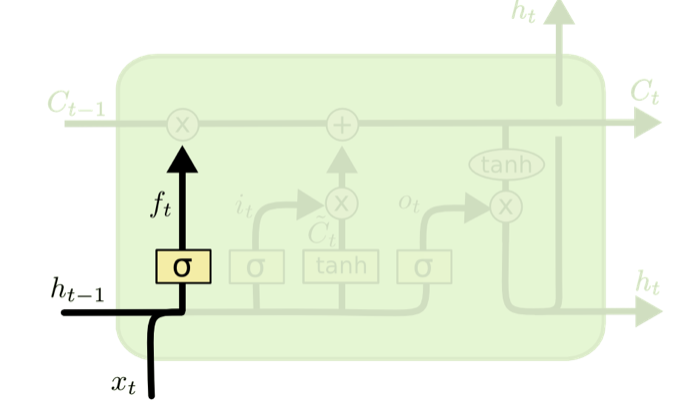
\includegraphics[width=80mm,scale=0.7]{lstms1}
	\caption{Forget layer in LSTM \cite{lstmsite}}
	\label{fig:lstms1}
\end{figure}
In a symmetric way, the input gate defines the values of the same concatenated vector to keep: $i_t=\sigma(W_i[h_{t-1};x_t]+b_i)$.\\Secondly, always at this level, a candidate cell state is built: $\widetilde{C_t}=tanh(W_c[h_{t-1};x_t]+b_c)$ (Fig. ~\ref{fig:lstms2}).
\begin{figure}[H]  \centering
	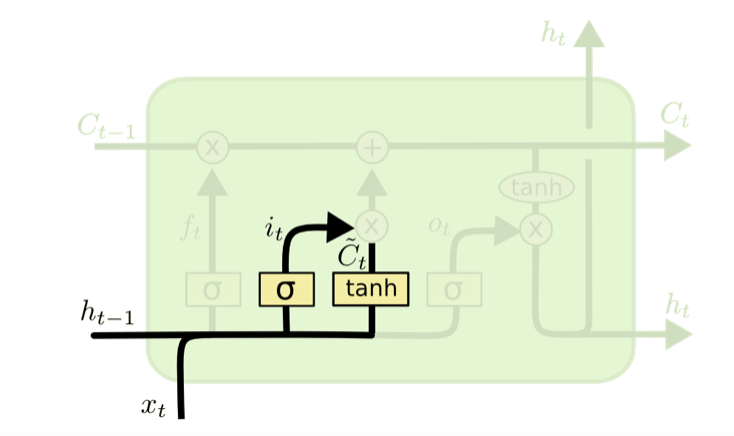
\includegraphics[width=80mm,scale=0.7]{lstms2}
	\caption{Input layer in LSTM \cite{lstmsite}}
	\label{fig:lstms2}
\end{figure}
It is clear now how to update the cell state: $C_t =f_t\cdot C_{t-1} + i_t\cdot \widetilde{C_t}$ (Fig. ~\ref{fig:lstms1}).
\begin{figure}[H]  \centering
	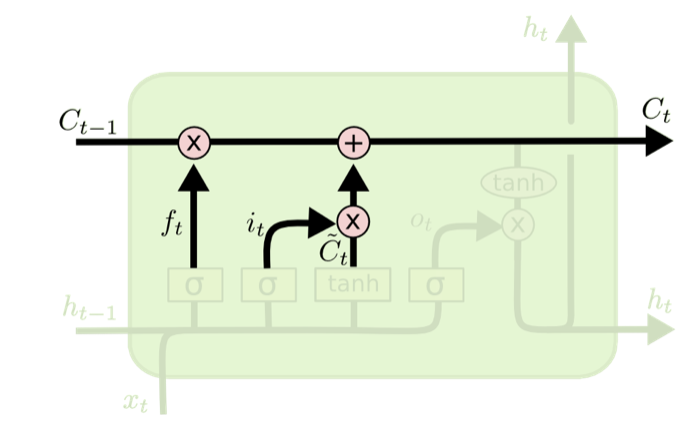
\includegraphics[width=80mm,scale=0.7]{cellupd}
	\caption{Cell update in LSTM \cite{lstmsite}}
	\label{fig:cellupd}
\end{figure}
Finally, the output gate will produce the output: $o_t = \sigma(W_o[h_{t-1};x_t]+b_o)$ and the hidden state: $h_t=o_t\cdot tanh(C_t)$ (Fig. ~\ref{fig:lstmout}).
\begin{figure}[H]  \centering
	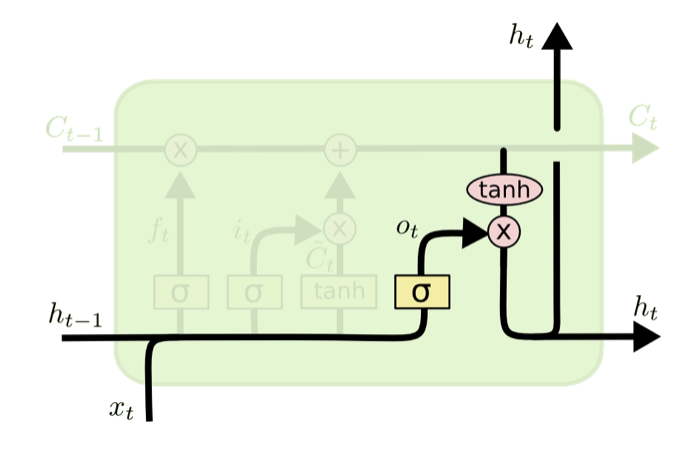
\includegraphics[width=80mm,scale=0.7]{lstm-out}
	\caption{Hidden state and output in LSTM \cite{lstmsite}}
	\label{fig:lstmout}
\end{figure}
The discussed structure is a valid solution to overcome the vanishing gradient problem. In fact, if we compute the recursive gradient in this case we have: $\frac{\partial C_t}{\partial C_{t-1}} = f_t + K$, where $K$ is the result of the other partial derivatives, that for our concern are not of interest.\\The crucial point here, is that even in case of long term dependency where we multiply the derivative previously computed several times, the term: $f_t$ can always assume any values in the range [0,1] and it does not exponentially converge to zero.\\In addition to this the presence of gates with internal parameters, instead of simple activation functions, allows the model to adaptively set the corresponding parameters with respect to the current input and hidden state. In this way the gates can actively update their state when the gradient is too low or too high.\\Finally, it is worth to note there are several variation on the described architectures.\\In 2002, it has been proposed a LSTM model (\cite{lstmv1}) where all the three gates:$G_1,G_2,G_3$ are conditioned by the cell state as well as hidden state: $G_i=\sigma(W_i[C_{t-1};h_{t-1};x_t]+b_i)$.\\Another variation that recently gained popularity is the Gated Recurrent Unit (GRU) (\cite{grupaper}). In the latter, the input gate is also used as forget gate: $f_t=1-i_t$. In addition to this, the cell and hidden states are merged together. Overall, we have:
\begin{enumerate}
\item $i_t=\sigma(W_f[h_{t-1};x_t])$: what to remember about the previous hidden state and input
\item $r_t=\sigma(W_r[h_{t-1};x_t])$: what to keep from the previous hidden state  
\item $\widetilde{C_t}=tanh(W [r_t\cdot h_{t-1};x_t])$: candidate hidden state (different from the candidate cell state in regular LSTM)
\item $h_t=(1-i_t)\cdot h_{t-1}+i_t\cdot\widetilde{C_t}$: the hidden state is built by forgetting about the previous hidden state and  adding what to remember about the candidate hidden state
\end{enumerate}
%step 1






 
\section{Attention}
Attention in neural networks aims to replicate the same human cognitive process. The latter is defined in \cite{psy}, as the behavioral process of concentrating on a portion of the total information while ignoring the rest: it is the allocation of limited cognitive resources.\\In the context of neural networks and predictions, attention allows to detect significant features during the training.\\Namely, it learns the filter to distinguish  between irrelevant, noisy inputs and remarkable one. Generally, attention is applied to Encoder-Decoder neural networks, to make explicitly the decoder knows where to look for the final prediction.
\subsection{Encoder-Decoder model}
Encoder-Decoder model is a general architecture constituted of two sequential blocks:
\begin{enumerate}
\item encoder that converts the input into a context vector. Basically, the encoder performs feature extraction.
\item decoder that takes the context vector and the previous output, to produce a final prediction. This is why it is autoregressive.
\end{enumerate}
Specifically, the layers in the encoder and decoder can be of any nature: for example image auto-encoders have Convolutional Neural Network (CNN) in the encoder and the analogous deconvolution in the decoder. Sequence to sequence tasks such as translation can have as encoder and decoder RNN or LSTM.\\It is essential to note the encoder turns the raw input into a suitable representation for the decoder.\\However, as the input's size increases the more difficult is for the encoder to correctly summarize it into a fixed-length vector. In addition to this, as it is the case of sequence to sequence task such as translation, the output should be conditioned not to the whole input sequence but only to a smaller useful portion.\\With attention the encoder does not need to produce a fixed-length vector, but it encodes the input into a sequence of vectors and adaptively chooses which of them are essential.\\Formally, the encoder-decoder model can be formulated as (\cite{bah}):
\begin{enumerate}
\item input sequence: $\textbf{x}=(x_1,\dots,x_{T_{x}})$, where $T$ is the length of the $x$-th input sequence
\item hidden states at time $t$: $h_t=f(x_t,h_{t-1})$ where $f$ can be for example an LSTM or CNN
\item context vector: $c=q(h_1,\dots,h_{T})$ where for LSTM $q=h_{T}$. In fact, with a recurrent encoder-decoder the context vector for the decoder input is the last encoder's hidden state
\item decoder's prediction at time: $t'$ is: $y_{t'}$ and it is conditioned to the previous output: $y_{t'-1}$ and context vector: $c$.
\end{enumerate}
It is important to note that $t'$ is the output sequence length that is not necessarily equal to the input length: $T$.\\Practically, the decoder defines the prediction as: $p(y_{t'}|(y_{t'-1},c,s_{t'})=g(y_{t'-1},c,s_{t'})$ where $g$ is the function implements the decoder block and $s_t$ is its internal state.\\Finally, the encoder part, before producing the context vector for the decoder can traverse the sequence in both ways (left/right and right/left) so that now each annotation is the concatenation of both hidden states : $h_j = [\overrightarrow{h_j},\overleftarrow{h_j}]$: Bidirectional RNN. In this way the context vectors model the relationship of a given word with the previous and following positions.

\subsection{Attention in Ecoder-Decoder}
The previously discussed formulation can be extended to attention, by conditioning the output at time $t'$: $y_{t'}$ not to a global context vector: $c$, but to a context vector that is specific for the given instant: $c_{t'}$.\\In particular we have that: $p(y_{t'}|(y_{t'-1},c_{t'},s_{t'})=g(y_{t'-1},c_{t'},s_{t'})$.\\Generally, $c_{i}$ is a weighted sum over all the hidden states of the encoder for a given sequence: $c_{i} = \sum_{j=1}^{T_x}\alpha_{ij}h_j$, where $\alpha_{ij}=\frac{exp(e_{ij})}{\sum_{k=1}^{T_x}exp(e_{ik})}$. Finally, the crucial step is how the alignment scores are computed: different attention algorithms mainly differs for this computation: $e_{ij}=a(s_{i-1},h_j)$. The latter measures how the previous hidden state of the decoder: $s_{i-1}$ is relevant to the encoder's hidden state: $h_j$.\\Basically, the context vector is a weighted sum over all the encoder's hidden states: $c_{i}$ and $\alpha_{ij}$ is a probability measure of how much $h_j$ is relevant for the previous decoder's internal state: $s_{i-1}$ for the following state and final prediction: $s_i$ and $y_i$ (~\ref{fig:encdecatt}).\\At the beginning of each sequence, the decoder state is initialized with the last hidden state of the encoder.
\begin{figure}[H]  \centering
	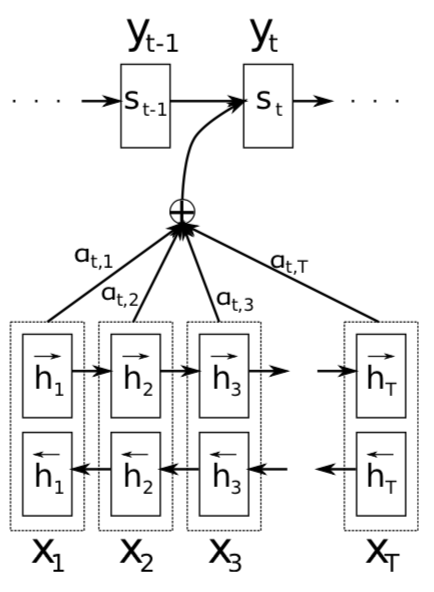
\includegraphics[width=40mm,scale=0.5]{encdecatt}
	\caption{Graphic representation of attention in RNN ecoder-decoder: \cite{psy}}
	\label{fig:encdecatt}
\end{figure}
In this way, the decoder select which part of the input hidden states to pay attention to.\\The encoder-decoder models performs this type of filtering also without attention but with a latent mechanism: on the opposite attention explicitly forces the decoder to focalize on relevant features.\\Finally, the attention vector that is the final output is obtained applying a dense layer to the concatenation of $c_t$ and $h_t$: $a_i=tanh(W[c_i;h_i])$
\subsection{Multiplicative and Addititive Attention}
There are two main mechanism to computer the attention scores:
\begin{enumerate}
\item Luong's multiplicative (\cite{luong}): $e_{ij} = h_{i}^{T}Wh_{j}$
\item Bahdanau's additive style (\cite{psy}): $e_{ij} = v_{a}^{T} \cdot tanh(W_{a}s_{i-1} + U_{a}h_j)$
\end{enumerate}
In the above definitions, $W,U,v_a$ are matrixes to be learned during the training: practically they are fully connected layers.\\The two methods have the same computational complexity but the first one is more efficient since it only requires matrix multiplications for which the GPU hardware is highly specialized.



\section{Transformer}
Transformer (\cite{aiayn}) is a neural network architecture introduced in 2017 by Google research, for Natural Language Processing (NLP). A series of experiments in NLP task have shown Transformer is better than classical approaches based on Recurrent Neural Networks (RNN), in terms of accuracy and computational efficiency.\\I have adapted this structure for arrhythmia detection since like NLP tasks, the input data is a collection of sequences  (heartbeats) and the information about the output is concentrated in the relationships between the sigle sequence's components ( millivolts sample).\\The main issue for NLP tasks such as translation is word sense disambiguation, namely the semantic of a term given its context in a phrase. RNN approaches this problem considering for each word, the previous hidden state.\\However, this sequential characteristic precludes parallelization within training samples because before predicting the actual hidden state we need to know the previous one. In addition to this, RNN has difficulties to learn dependencies between distant words.The Transformer solves this problems using non recurrent layers and self attention.\\It has an encoder-decoder structure. Specifically, the encoder is made of 6 identical layers. Each of them consists of two consecutive residual blocks where the first one is the self attention layer, while the second one is a fully connected layer: they are both followed by a normalization layer.\\The decoder is equal to the encoder, except for the presence of an additional self attention layer (~\ref{fig:tramodel}).
\subsection{Transformer's Attention}
The essential transformer's layer is the multi head attention. I will first describe the low dimensional case and secondly the multi head approach.\\As we said before, the input is a sequence where each component has in total: $d_k$ features because as it is the case of NLP, the input is followed by an Embedding Layer.\\Initially, it applies to each component three different dense layers to obtain respectively: Query ($Q$), Key ($K$), Value ($V$) vectors.\\Secondly, for each position in the sequence, it compares the associated component against each other to obtain a score of how much a given input is expressed in that position: $A = softmax(\frac{QK^T}{\sqrt(d_k)})$.\\Finally, all the value vectors are weighted summed considering the latter score, to obtain the output vector in that position: $Attention(Q,K,V) = AV$. This type of attention is dot-product attention and it is faster than additive attention, because the described multiplications can be computed with optimized vectorial operation. The role of $d_k$ is required to avoid the vanishing gradient, caused by high values in the $softmax$ argument: without $d_k$, the longer input sequences the higher is: $QK^T$, and the lower will be the gradient of the $softmax$.\\The drawback of this approach is related to the fact that when computing the scores of a component with all the others, the higher score will be presumably related to the actual input itself.\\To overcame this issue, the paper introduces the multi head attention, where basically the attention vectors are computed $h$ times (or head) with a different triple of matrixes $W^{Q}_{i},W^{K}_{i},W^{V}_{i} \; \forall 0\leq i\le h$.\\In this way, the model learns the importance of a given component from different representation subspaces at different positions, because each head can learn different relationships. Specifically, it performs the following operation: $MultiHead(Q,K,V)=Concat(head_1,\dots,head_h)W^O$ where $head_i= Attention(QW_{i}^{Q} , KW_{i}^{K} , VW_{i}^{V} )$ (Fig. ~\ref{fig:mhsa}).
\begin{figure}[H]  \centering
	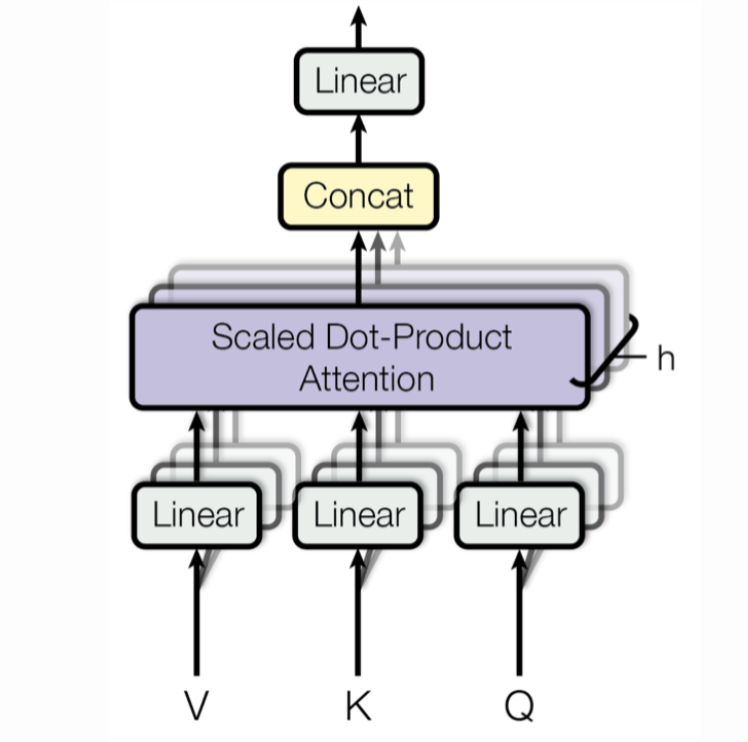
\includegraphics[width=80mm,scale=0.7]{mhsa}
	\caption{Multi Head Attention: \cite{aiayn}}
	\label{fig:mhsa}
\end{figure}
The above operations are independent of the sequence length so that the computational cost is constant while RNN needs to iterate over all the sequence's components. It can be parallelized since each single attention vector can be computed independently.\\Finally, the scores between sequence's components does not depend on the distance while RNN fails to model relationships between distant input.
\begin{figure}[H]  \centering
	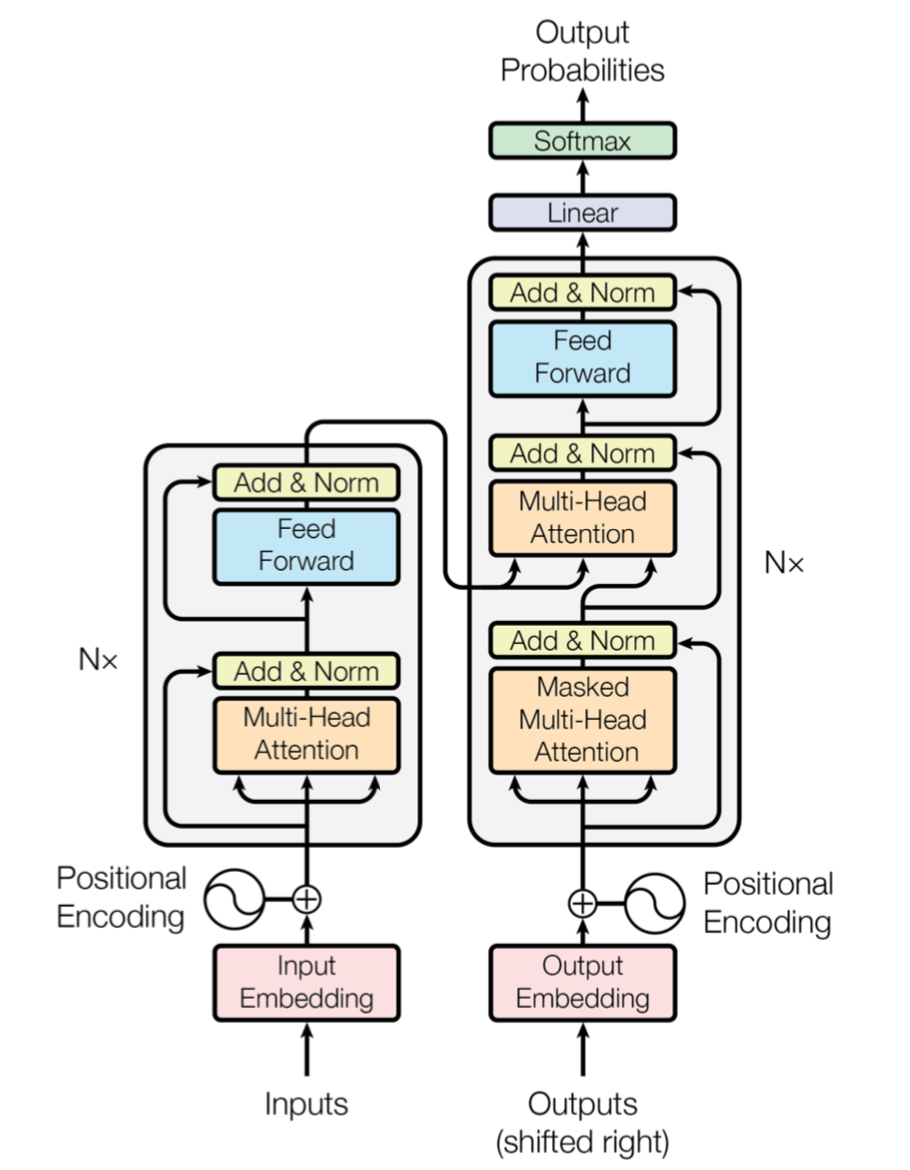
\includegraphics[width=80mm,scale=1]{transflay}
	\caption{Transformer model: \cite{aiayn}}
	\label{fig:tramodel}
\end{figure}
\section{Neural Ordinary Differential Equations}
Neural Ordinary Differential Equations (NODE) (\cite{DBLP:journals/corr/abs-1806-07366}) have been awarded as best paper in NeurIPS 2018 . In the following, I will describe first the Residual Neural Networks (ResNet), since NODE are the direct successor.
\subsection{Residual Neural Network}
ResNets (\cite{DBLP:journals/corr/HeZRS15}) have been introduced after verifying the consequences on neural networks performance, when more layers are added.\\The interest in this argument is justified by the presence of very deep neural networks that perform well on challenging dataset such as the ImageNet dataset (\cite{Simonyan14verydeep}).\\Basically, the argument is if increasing the depth of a neural network, always the optimal choice to improve its performance. Vanishing gradient is an issue related to deep models, but it can be solved using normalization techniques. The paper's response to the above problem is negative.\\The authors made a series of experiments and verified deep neural networks experience the degradation problem: with the depth increasing, accuracy on the test set does not improve and the culprit is not overfitting.\\The degradation problem shows not all systems are similarly easy to optimize (\cite{DBLP:journals/corr/HeZRS15}): deeper model can lead to higher error both on training and test set.An example of the above issue is visible if we add identity layers to a neural network. We should except no loss in accuracy than the shallower counter part, but in practice the opposite is true. ResNets are introduced to solve the degradation problem.\\A single residual block turns the input: $x$ into the output: $Y$: through the formula: $Y = x +F(x)$: $F$ is a generic function implemented as multiple stacked neural network layers (~\ref{fig:resnetfunc}).
\begin{figure}[H]  \centering
	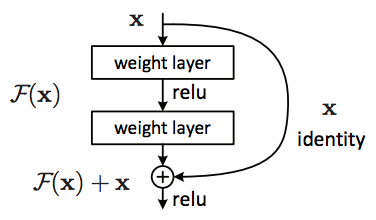
\includegraphics[width=80mm,scale=0.7]{resnetfun.png}
	\caption{Graphic representation of a residual block}
	\label{fig:resnetfunc}
\end{figure}
In this context, a ResNet with N residual blocks can be modeled as : $Y_{i+1} = Y_{i} +F(Y_{i},\theta_{i}) \forall i \in [1,..,N]$, where $\theta_{i}$ are the weights of the $i-th$ layer to be learned.\\ResNet are different from Feed Forward Network (FNN) because: FNN maps the input : $x$, to the output $Y$, with multiple stacked hidden layers : $h_1, \dots, h_n$, so that the objective of the learning is a direct mapping from input to the output : $Y=h_n(\dots (h_1(x))$.\\On the opposite a single residual layer maps the input to the output specifying a function $F$ that instead of learning a direct maps between input and output, models the difference between them because the hypothesis is that it is easier to optimize the residual mapping than to optimize the original, unreferenced mapping (\cite{DBLP:journals/corr/HeZRS15} ).\\The reason why ResNet solves this problem has been verified in \cite{DBLP:journals/corr/HeZRS15}. and the explanation is that for the model it would be easier to set to zero the residual function, rather than learning the identity mapping through non linear activation functions.\\In practice, the identity mapping is not the optimal one. However, it should be more feasible for the solver to find the perturbations with reference to an identity mapping, than to learn the function as a new one (\cite{DBLP:journals/corr/HeZRS15} ).\\This last consideration is a crucial similarity between ResNet and NODE: David Duvenaud (author of \cite{DBLP:journals/corr/abs-1806-07366}), explains in a forum that the idea behind NODE is the intuition it is easier to model a small change to an almost-correct answer than the whole improved answer at once.\\In Fig.~\ref{fig:degprob}, thin and bold curves denote respectively the training and validation error on ImageNet dataset. It is visible how on a plain neural network (on the left), more layers cause higher training/validation error, while deeper ResNet (on the right) have better performances.
\begin{figure}[H]  \centering
	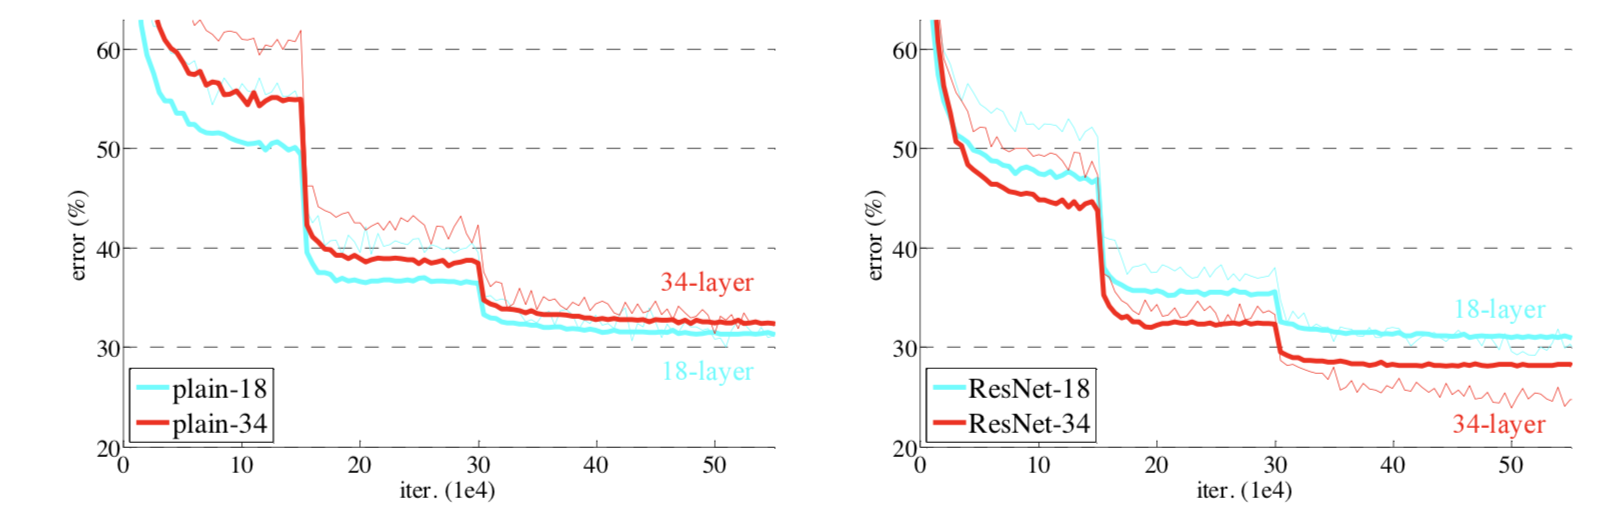
\includegraphics[width=100mm,scale=0.7]{degprob.png}
	\caption{Comparison of plain and residual neural networks (\cite{DBLP:journals/corr/HeZRS15})}
	\label{fig:degprob}
\end{figure}
\subsection{NODE}
The connection between ResNet and NODE is the interpretation of ResNet as differential equation. In particular, from the definition of ResNet previously discussed, we can relax the constraint that $i$ is a discrete value, by gradually reducing the step size: $[i,i+1]$.\\For example we could take half of the original step and rewrite the relationship as: $Y_{i+0.5} = Y_{i} +F(Y_{i},\theta_{i}$, so that: $Y_{i+1} = Y_{i+0.5} +F(Y_{i+0.5},\theta_{i+0.5} = Y_{i} + F(Y_{i},\theta_{i} + F(Y_{i+0.5},\theta_{i+0.5})$.\\The latter equation shows reducing the step-size to the half is equivalent to double the number of residual layers in the discrete case. In the limit, if we take smaller steps and add more layers, it is possible to describe the dynamic of the ResNet as an initial value problem where: 
\begin{enumerate}
\item $F(Y(t),\theta_{t},t)$ = $\frac{\partial Y(t)}{ \partial t}$ is an ordinary differential equation
\item $Y(0)=Y_0$ is the input data, namely the initial condition
\item $T$ is the evaluation time 
\end{enumerate}
In particular, the NODE output at time $T$ is obtained using an ODE-solver, where it is possible to specify the maximum approximation in terms of a scalar: $e$. To summarize, in a NODE block we specify the respective output as the solution of a ODE problem.\\The main difficulty to train this structure is that performing back-propagation through the ODE solver requires high memory cost and introduces additional numerical error (\cite{DBLP:journals/corr/abs-1806-07366}).\\To solve this issue the authors propose the Adjoint method that scales linearly with problem size, has low memory cost, and explicitly controls numerical error, whose implementation is written in PyTorch and available on GitHub.\\It is important to note that the depth of a NODE is not a clear concept because $t$ is now real value, not an integer as it is the case of ResNet.However, the number of function  evaluation to solve the differential equation during the forward pass of the NODE can be considered as an estimation of the complexity of the  model.\\The benefits of NODE are the following :
\begin{enumerate}
\item Memory efficiency because to train the model it is not required to store the intermediate forward output at every layer, that normally it is used by the back propagation algorithm to compute the gradients of the weights of each layer.
\item Adaptive computation because the time complexity of the ODE solver depends on the error accuracy specified and the ODE solver can adapt their strategy on the fly on the basis of that accuracy.  In addition to this after the model has been trained with a given tolerance, it can be tested and used in production with a lower error tolerance so that it is faster and less intensive (useful for embedded device)
\item Parameter efficiency because parameters of nearby layers are automatically tied together (\cite{DBLP:journals/corr/abs-1806-07366})
\end{enumerate}
\begin{figure}[H]  \centering
	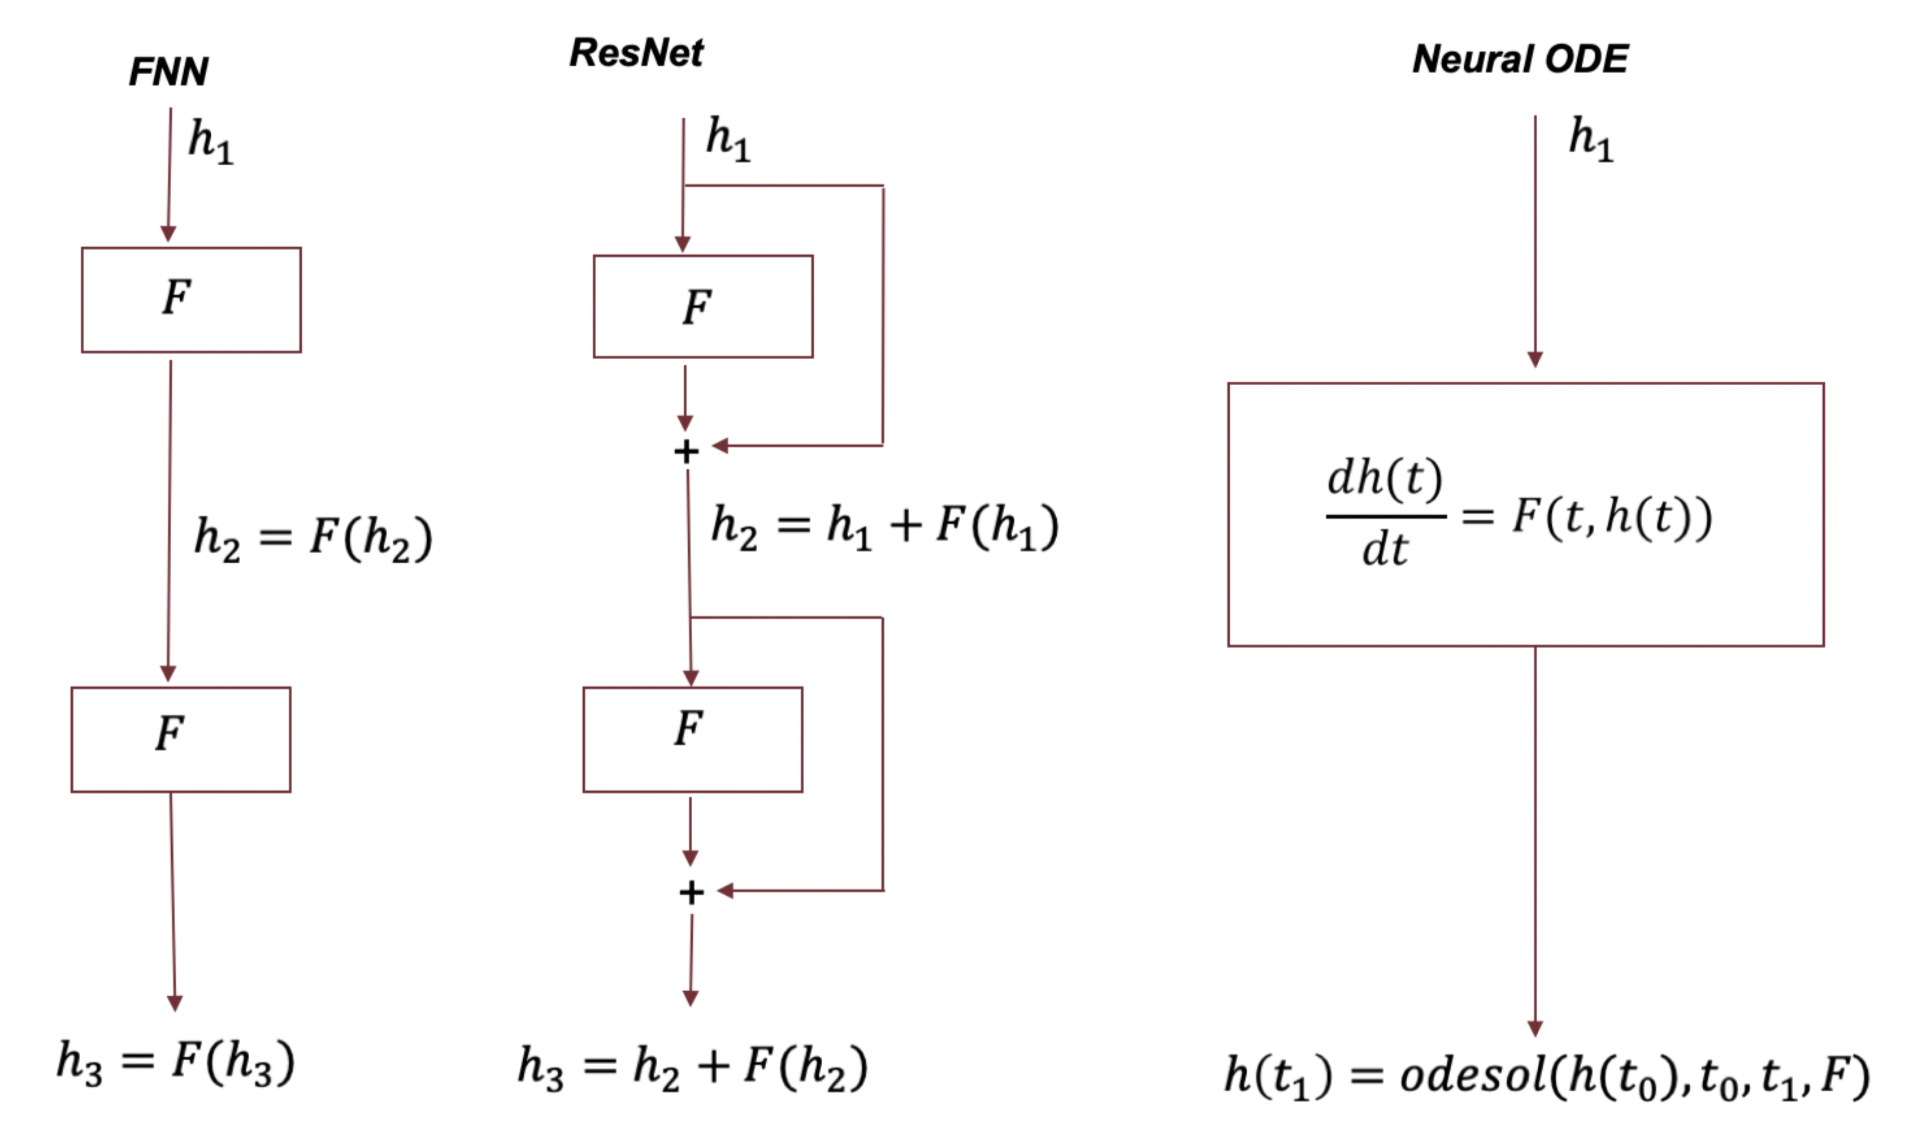
\includegraphics[width=100mm,scale=0.7]{cmplink.png}
	\caption{Comparison of FNN, ResNet, NODE}
	\label{fig:cmplink}
\end{figure}
I will conclude this section describing the connection between NODE and ResNet in terms of ODE approximation. The characteristic equation of a residual block is: $Y_{i+1} = Y_{i} +F(Y_{i})$ and it can be interpreted as the Euler approximation of $\frac{\partial Y}{\partial i} = F(i)$ at time $i$ with unitary step size. NODE instead approximate the same function using more accurate ODE solver than the Euler method (Fig.~\ref{fig:eulermethod}). 
\begin{figure}[H]  \centering
	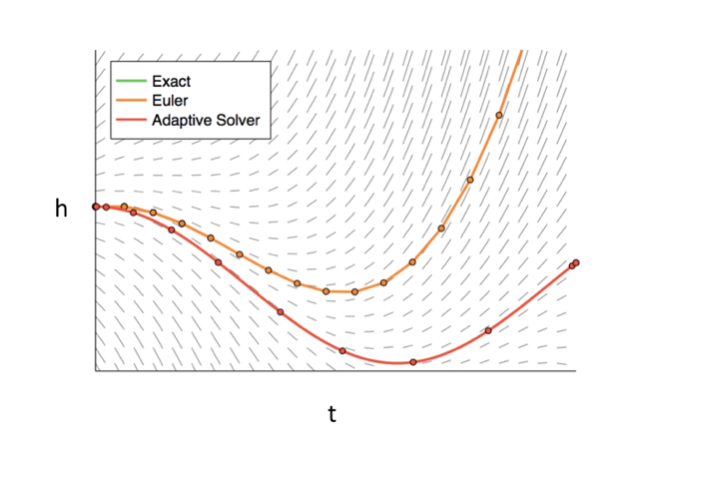
\includegraphics[width=80mm,scale=0.7]{eulermethod.png}
	\caption{Comparison of Euler method (orange), NODE solver (red) to approximate  $\frac{\partial Y}{\partial i} = F(i)$. The latter coincides with the NODE solution }
	\label{fig:eulermethod}
\end{figure}
\chapter{Experiment}

\section{Dataset}
The database considered in this study is a collection of annotated ECG recordings obtained by the Arrhythmia Laboratory of Boston's Beth Israel Hospital, known as the \textit{MIT-BIH Arrhythmia Database} (\cite{dbmitbih}).\\I contains 48 half-hour excerpts of two-channel ambulatory ECG recordings, obtained from 47 subjects studied by the BIH Arrhythmia Laboratory between 1975 and 1979.\\The recordings are obtained with a frequency of 360 Hz: this means each recording approximately consists of: $30\cdot360=10800$ samples.\\Two or more cardiologists independently annotated each record for a total of 110,000 annotations included with the database: it is is worth to mention, each annotation is placed in correspondence to the R peak of a single beat, so that we have implicitly solved for this specific case the beat detection problem.\\According to the Association for the Advancement of Medical Instrumentation (AAMI) standard (\cite{aamistd}) for testing and reporting performance results of cardiac rhythm and segment measurement algorithms, the evaluation of an arrhythmia detector algorithm should be made on the classification performance on five major categories of heartbeats:
\begin{enumerate}
\item N: includes beats originating in the sinus node (normal and bundle branch block beat types)
\item S: includes supraventricular ectopic beats (SVEBs);
\item V: includes ventricular ectopic beats (VEBs);
\item F: includes beats that result from fusing normal and VEBs;
\item Q: includes any heartbeat not in the N, S, V or F categories, essentially the undefined heartbeats as well as beats resulting from the use of a pacemaker.
\end{enumerate}
The last category includes beats that are a result of a pacemaker operating under the skin of the patient.\\These beats are regulated and it is not meaningful to use them for arrhythmia classification: this is why  we excluded all these beats from our study.\\Please note also that this is a common practice followed by other studies in the state-of-the-art(\cite{fog}). Therefore, we are left with four beat categories.\\A more detailed topology of the dataset is depicted in Fig.~\ref{fig:aamiimg}.
\begin{figure}[H]  \centering
	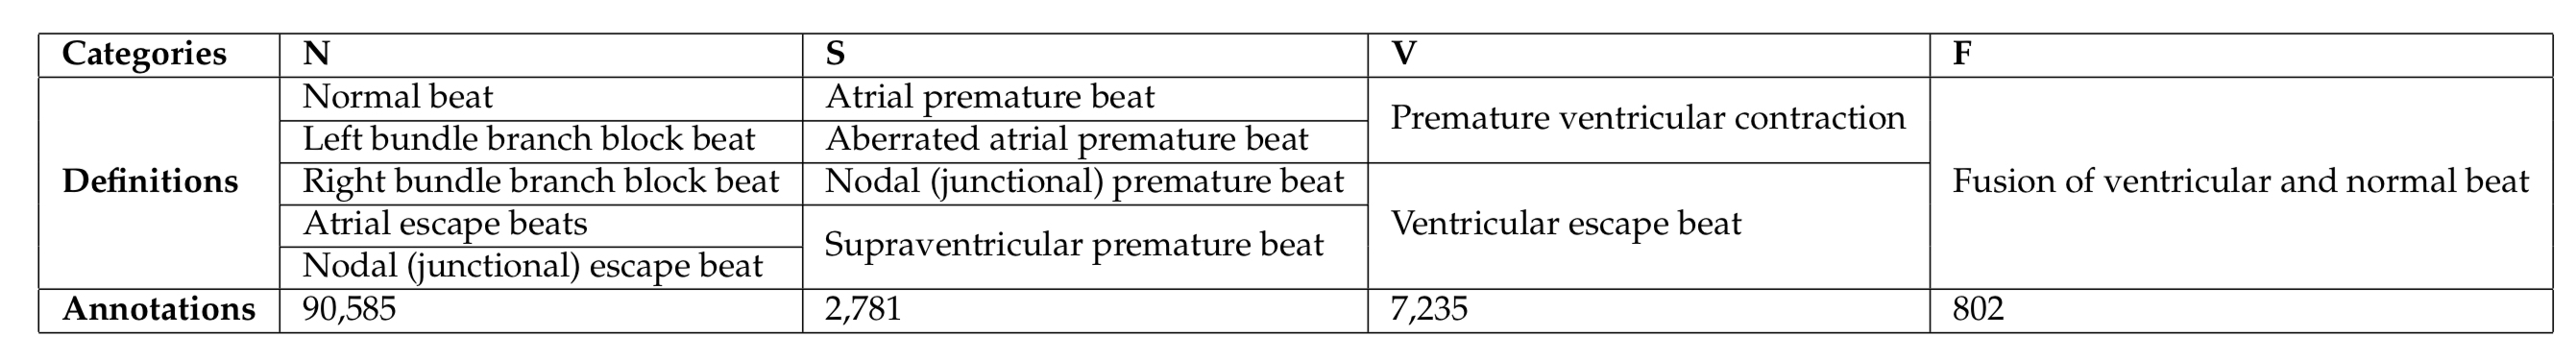
\includegraphics[width=150mm,scale=0.7]{aamiimg}
	\caption{AAMI 5 categories of heartbeats  (\cite{aamistd})}
	\label{fig:aamiimg}
\end{figure}
It is clear how the N class is more populated than the others: it constitutes the $89\%$ of the whole dataset. This overbalancing can lead to an inconsistent training and poor quality algorithms. In order to mitigate the latter we have adopted data augmentation techniques such as ADASYN and SMOTE, and a weighted loss function. The latter is intended to give higher weight and consequently penalize more the misclassification error due to under represented samples.


\subsection{Training and Test Set}
We have considered two dataset configuration. In the first one, we have built the test set, by randomly choose from the dataset the following samples:
\begin{enumerate}
\item N: 900
\item S: 900
\item V: 900
\item F: 250
\end{enumerate}
In a second configuration we wanted to test the robustness of our algorithms: we decided to create personalized classifiers for the patients: 222,223,233.\\In detail, we first trained a model on the whole dataset without the latter three patients.\\Secondly, for each single patient we have built the test set in the following way.\\Patient 222:
\begin{enumerate}
\item N: 50 from 2273
\item S: 20 from 209
\item V: 0 (this patient does not have beats labeled as V)
\item F: 0 (this patient does not have beats labeled as F)
\end{enumerate}
Patient 223:
\begin{enumerate}
\item N: 50 from 2045
\item S: 20 from 73
\item V: 100 from 473
\item F: 5 from 14
\end{enumerate}
Patient 233:
\begin{enumerate}
\item N: 500 from 2229
\item S: 2 from 7
\item V: 250 from 830
\item F: 2 from 11
\end{enumerate}



\section{Performance Measures}
In a classification problem with N classes: ${C_1,\dots,C_n}$, it is possible to determine the quality of the classifier, in terms of $C_{i,j}$, that is the number of dataset's samples belonging to $C_i$ , but predicted as $C_j$, where $1 \leq i,j \leq n$.\\In particular given a generic class: $C_i$, we define:
\begin{enumerate}
\item True Positive (TP): $C_{i,i}$%$\sum_{i=1}^{n}$
\item False Positive (FP): $\sum_{j\neq i}C_{j,i}$
\item False Negative (FN): $\sum_{j\neq i}C_{i,j}$
\end{enumerate}
%A confusion matrix: $M$, contains the described parameters: it is $n\cdot n$ and $M_{i,j}=C_{i,j}$
The performance metrics we have used are:
\begin{enumerate}
\item Precision: $\frac{TP}{TP+FP}$
\item Recall: $\frac{TP}{TP+FN}$
\item F-score: $2\cdot \frac{Precision\cdot Recall}{Precision+Recall}$
\end{enumerate}
It is significant to note the trade-off between precision and recall: if the model predicts all the samples as belonging to a given class it will reach a recall of 100\% because no sample will be classified with a different label. Consequently, the false negative will be zero. On the other hand in this situation, the number of wrongly classified samples ($FP$) will be high and consequently the precision low.\\In order to plot precision and recall for all the classes, it is possible to use the confusion matrix: $M$: it is $n\cdot n$ and $M_{i,j}=C_{i,j}$



\section{Random Forest \cite{forest}}
The paper (\cite{forest}) performs  a different classification task since it does not predict the 5 classes specified by the the (AAMI) standard, but the following different labels : N, L, R, V, P, described in the MIT-BIH annotations (Fig.~\ref{fig:allclass}).\\Even if this is a different task, I have decided to replicate it, because the approach is straightforward and performs well.\\In this way, I was able to concentrate on dataset building and fix some bug in the beat extraction.\\In addition to this, I could immediately re-adapt it to the original problem and infer the main issues of our dataset, and find more appropriate solutions.
The algorithm consists of three steps:
\begin{enumerate}
\item pre-processing: remove noise from the ECG signal
\item processing: heartbeat detection and feature extraction with DWT
\item classification: this is the first approach in literature to use Random Forest for arrhythmia classification
\end{enumerate} 
The ECG signal is first de-noised with a median filter, to remove baseline wandering. Recall that the latter is noise due to patient movement during the ECG recording.\\In Fig.~\ref{fig:rf1}, there is the application of the median filter: it is visible how the filtered signal is translated among a common axis. 
\begin{figure}[H]  \centering
	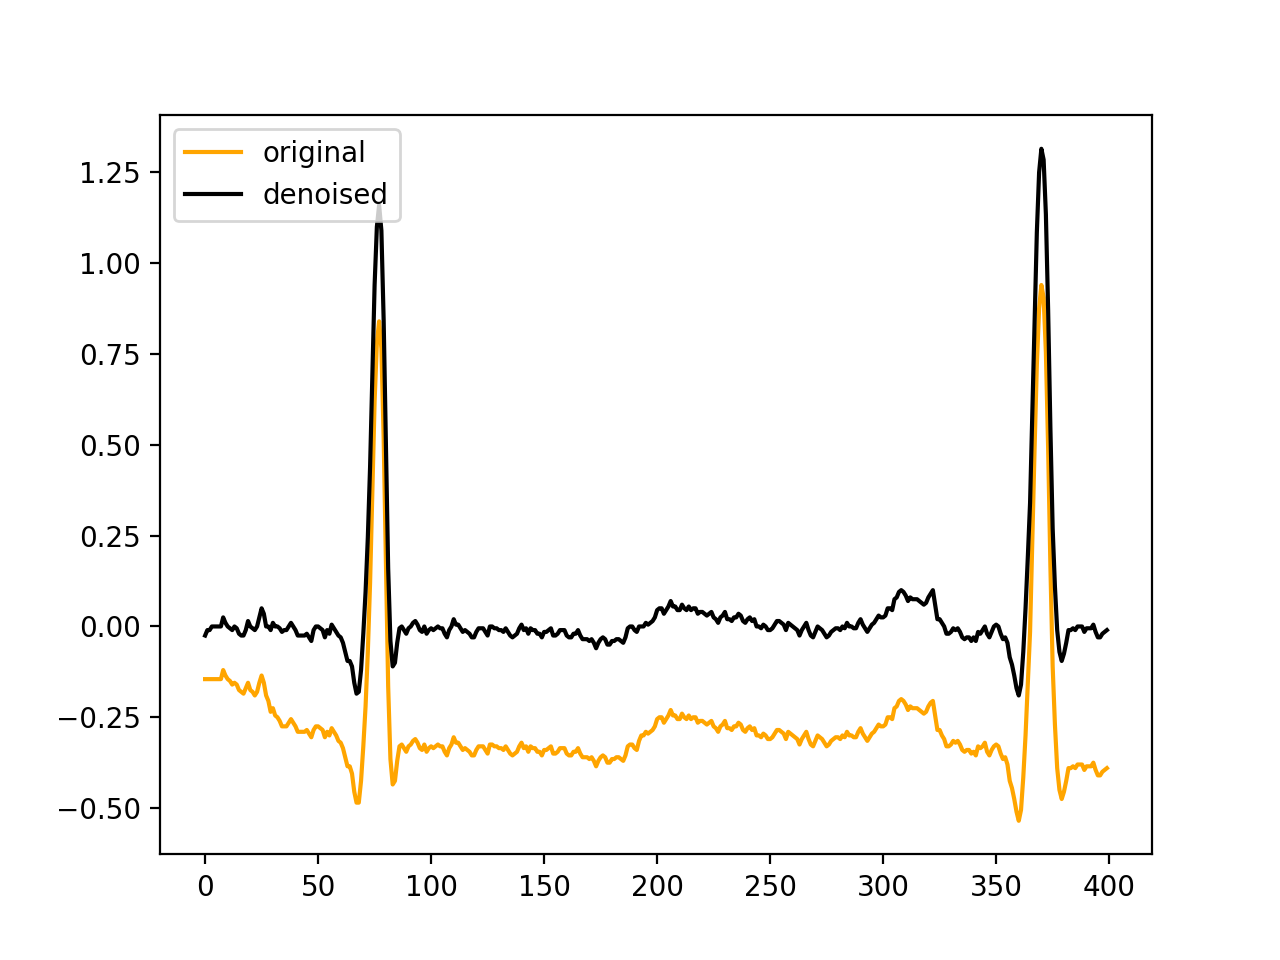
\includegraphics[width=80mm,scale=0.7]{random-forest-before-after}
	\caption{A fragment of ECG before and after the median filter}
	\label{fig:rf1}
\end{figure}
Each beat is defined as a sequence of 256 samples in the RR interval.\\To extract relevant features, they applied DWT and precisely Daubechies db2 wavelet because it gives better accuracy than other wavelet such as Symmlet sym6 and Symmlet sym10.\\Specifically, for each beat, the DWT is applied considering the first 4 levels of details coefficients (129+66+34+18 coefficients) and the fourth level of approximation coefficients (18 coefficients), for a total of 265 features per beat.\\The training set is made of 240 samples for each class and the test set of 120 for each.\\The algorithm as said before is Random Forest.\\In Fig.~\ref{fig:rf2}, the confusion matrix plots the performance of this approach: it is almost perfect and this justified our attempt to use this approach for the original task: discussed in the following section
\begin{figure}[H]  \centering
	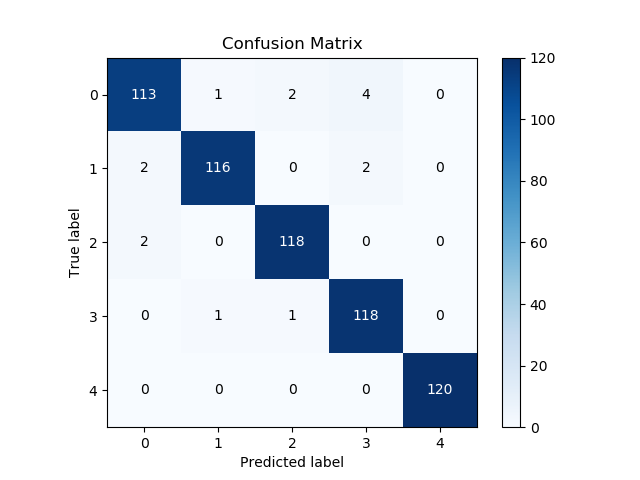
\includegraphics[width=100mm,scale=0.7]{confusion-matrix-dwt-random-forest-paper.png}
	\caption{Confusion Matrix : random forest for the N,L,R,V,P classification}
	\label{fig:rf2}
\end{figure}
\subsection{Custom Variation}
Initially, we have applied the same technique to the original problem with N,S,V,F classes. In Fig.~\ref{fig:rf3}, it is possible to see the accuracy metrics.
% ok
\begin{figure}[H]  \centering
	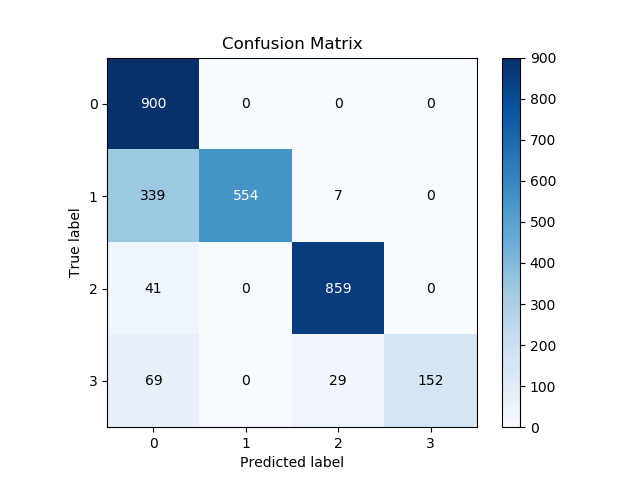
\includegraphics[width=100mm,scale=0.7]{random-forest-no-aug.png}
	\caption{Confusion Matrix : random forest without data augmentation for the N,S,V,F classification}
	\label{fig:rf3}
\end{figure}
It is clear how this modification in the dataset, determined a consistent drop in accuracy with respect to the previous problem.\\Primarily, this is due to the fact, our dataset is overbalanced and this is why we applied SMOTE and ADASYN (Fig.~\ref{fig:rf4}) to make it more uniform.
% ok
\begin{figure}[H]  \centering
	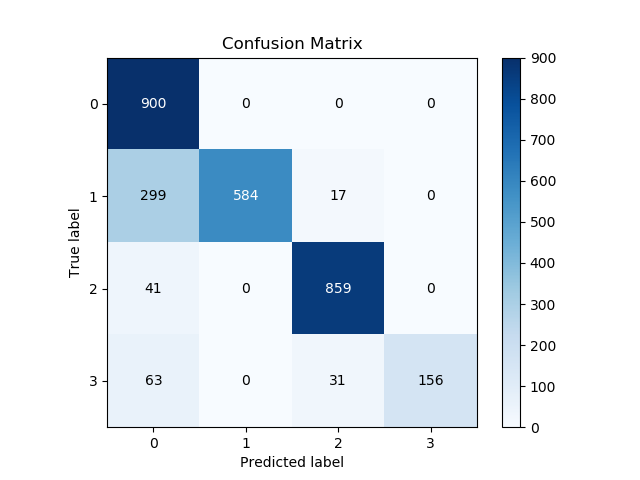
\includegraphics[width=100mm,scale=0.7]{random-forest-smote.png}
	\caption{Confusion Matrix : random forest after data augmentation for the N,S,V,F classification}
	\label{fig:rf4}
\end{figure}
The benefits of SMOTE and ADASYN for the model are completely the same and in general the overall performance are still low.\\This is caused by the fact the N,S,V,F classes are macro-categories that consist of multiple single beat types: in the original paper the classes were single type so that it was easier for Random Forest to detect the relevant features.\\In order to solve the latter, we have opted for more complex algorithms, described in the following sections.


\section{Support Vector Machine \cite{svmnl}}
This paper (\cite{svmnl}) describes a valid solution to our classification problem with the four AAMI classes. As it is the case of the previous algorithm (\cite{forest}), from an high level perspective it is divided into pre-processing, processing and classification.\\In this case, the paper performs an initial phase of QRS-complex detection using the Pan-Tompkins algorithm. However, I have not implemented this step, because as I said in the introduction, I will directly consider the R peak annotation already present in the dataset.\\During the pre-processing phase, the de-noise is realized using the DWT: Daubechies db6 with nine levels: the signal is reconstructed considering only the details coefficients from level three to nine.\\In this way, the frequency ranges from 0 to 0.351 Hz and 45-180 Hz are not considered because the first one are linked to baseline wander and the latter does not contain useful information for arrhythmia detection.\\Each beat is a sequence of 200 samples centered in the R peak location.\\In Fig.~\ref{fig:svc1}, is visible how the DWT makes the original ECG signal more smooth and less affected from noise.
\begin{figure}[H]  \centering
	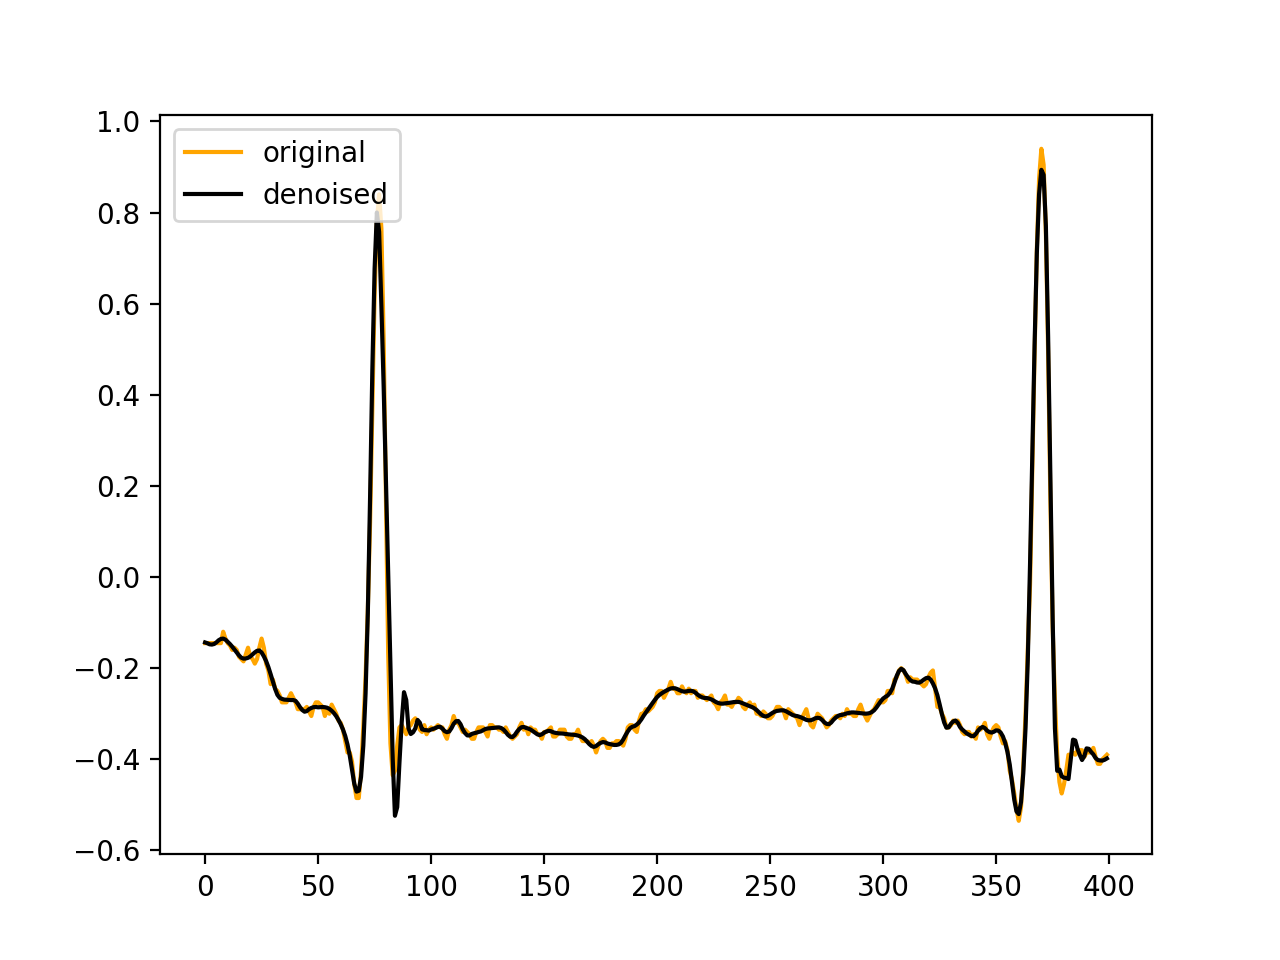
\includegraphics[width=80mm,scale=0.7]{svm-before-after}
	\caption{A fragment of ECG before and after the DWT}
	\label{fig:svc1}
\end{figure}
During the processing step, DWT,PCA,HOS and ICA are used.\\Initially, the DWT: Mayer with 4 levels is 
applied on each single beat to obtain the approximation coefficients in the range: 0 to 11.25 Hz. From that values, it considers only the third and fourth sub-bands for all the beats and consequently it creates respectively two matrices.\\Secondly, we apply PCA on each of the two matrices with 6 components, so that now we have 12 features per beat.\\Next, from each original beat of 200 samples, it applies $4_{th}$ and $5_{th}$ moment to each single beat to obtain two more features per beat.\\Finally, ICA with 14 components is applied to the matrix of beats, for a total of 28 features per beat.\\For the classification, it is used Support Vector Machine with the following parameters:
\begin{enumerate}
% SVC(C=70,gamma=0.7,kernel='rbf',verbose=True)
\item C: 70
\item Gamma: 0.7
\item Kernel: radial basis function
\end{enumerate}
The results, I have obtained are described in Fig.~\ref{fig:svc2}: we have comparable performances with respect to the previous algorithm based on Random Forest.
\begin{figure}[H]  \centering
	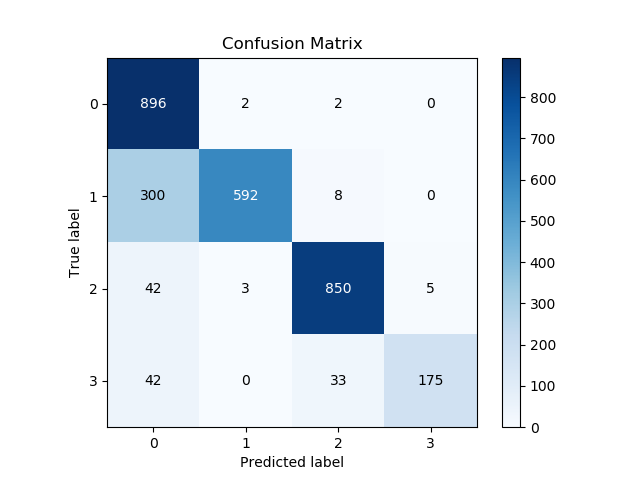
\includegraphics[width=100mm,scale=0.7]{confusion-matrix-linear-not-linear-no-aug-smaller-test.png}
	\caption{Confusion Matrix : svm for the N,S,V,F classification}
	\label{fig:svc2}
\end{figure}
We have tested the same approach applying data augmentation with ADASYN, obtaining slightly better results (Fig.~\ref{fig:svc3}).
\begin{figure}[H]  \centering
	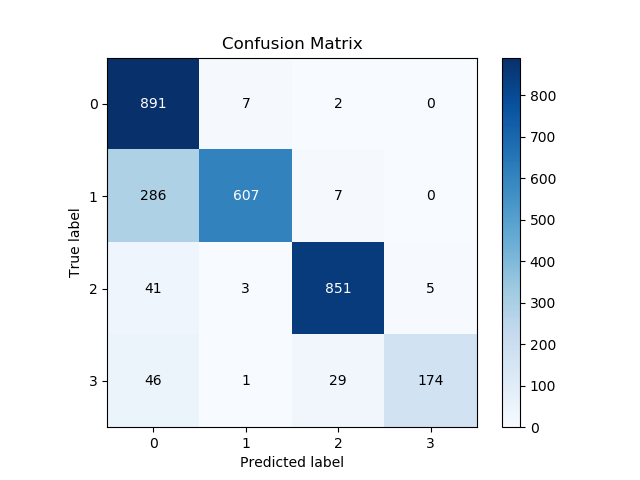
\includegraphics[width=100mm,scale=0.7]{confusion-matrix-linear-not-linear-adasyn-smaller-test.png}
	\caption{Confusion Matrix : svm with adasyn for the N,S,V,F classification}
	\label{fig:svc3}
\end{figure}
\section{Convolutional Neural Network  \cite{cnnfazeli}}
This paper (\cite{cnnfazeli}) describes an effective approach to solve two problems: arrhythmia classification and myocardial infraction.\\In particular the idea is to use a neural network to solve the first task and then apply transfer learning for the latter. Since we are only interested in arrhythmia detection, I will not discuss only the first part.\\The main difference of this solution with respect the previous two is that it does require a simple pre-processing phase without any de-noise procedure.\\Specifically, the latter consists of a first resample of the signal from 360Hz to 125Hz.\\Then, in order to find the R-peaks, it considers a temporal windows of 10 seconds, normalizes it and finally detects the R peaks as local maximum points above a threshold of 0.9.\\Secondly, it considers $T$ as the median of the RR peak distances in time for a given signal.\\Finally, each beat consists of R peak and the samples in the temporal segment of: $1.2 \cdot T$. Since $T$ is specific for a given signal, to make all beats of the same size, shorter beats are padded with zeros.\\The whole pre-processed dataset is available on Kaggle by the same author's paper, so I have not directly implemented this pre-processing.\\The algorithm for the classification is a neural network with one dimensional convolutional layers each with 32 kernels of size 5.\\In addition to this, it has max polling layers of size: 5 and stride: 2.\\The latter layers are arranged in a residual block the is repeated five times.\\At the end there are two fully connected layers followed by a $softmax$ (Fig.~\ref{fig:svc2}).(Fig.~\ref{fig:arch-cnn}).
\begin{figure}[H]  \centering
	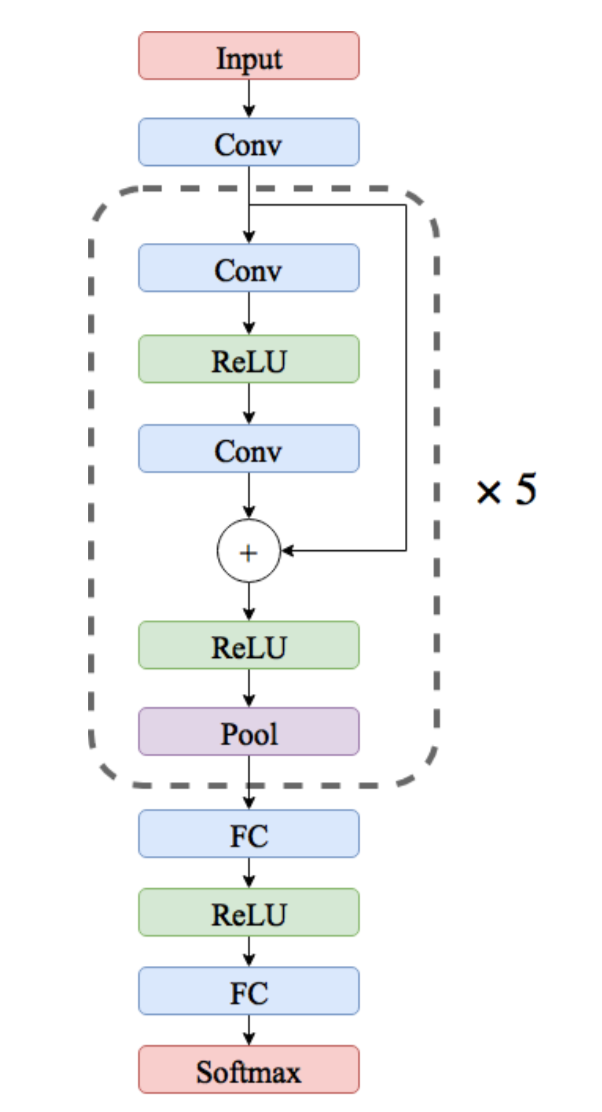
\includegraphics[width=50mm,scale=0.7]{arch-cnn}
	\caption{Architecture of the model in \cite{cnnfazeli}}
	\label{fig:arch-cnn}
\end{figure}
As loss function, it is used cross entropy with logits since the network's output is obtained with a $softmax$ and it can be interpreted as a probability distribution.\\The optimization method is Adam with the following parameters:
\begin{enumerate}
\item learning rate: 0.001
\item beta-1: 0.9
\item beta-2: 0.999
\end{enumerate}
It is employed an exponential learning rate decay, where the learning rate is decayed of 0.75 every 10000 iterations.\\I have implemented it in TensorFlow with Colab and trained it for 70 epochs.\\In Fig.~\ref{fig:cnn1}, I have plotted my results: they are not as good as the one described in the paper: I think this is due to the fact the latter does not describe the data augmentation technique used.
\begin{figure}[H]  \centering
	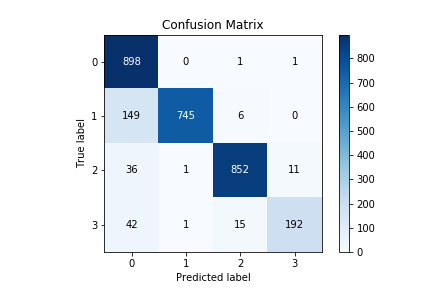
\includegraphics[width=100mm,scale=0.7]{cnn-no-data-aug.png}
	\caption{Confusion Matrix : cnn for the N,S,V,F classification}
	\label{fig:cnn1}
\end{figure}
We have tested the same approach using ADASYN as data augmentation (Fig.~\ref{fig:cnn2})
\begin{figure}[H]  \centering
	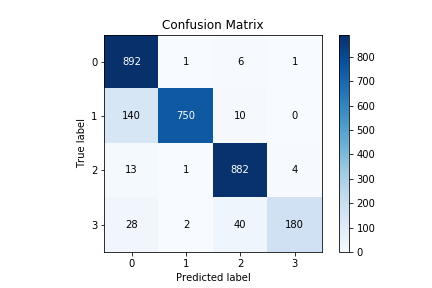
\includegraphics[width=100mm,scale=0.7]{cnn-adasyn.png}
	\caption{Confusion Matrix : cnn with adasyn for the N,S,V,F classification}
	\label{fig:cnn2}
\end{figure}
This approach has the benefit to have a simple pre-processing phase and it is conventional in the use of a neural network model that can be deployed in an embedded device with the support of library such as Tensorflow-Lite and uTensor.\\Finally, it has a better performance than the approach with Random Forest and Support Vector Machine.
\section{Neural Ordinary Differential Equations}
In this section I will demonstrate the application of NODE (\cite{DBLP:journals/corr/abs-1806-07366}) for arrhythmia detection: this is an innovative approach never used before in the literature.\\In order to implement it, I have adopted the PyTorch library provided by the same authors. The latter not only provides (ODE) solvers but also the optimized back-propagation using the adjoint method. In addition to this it has fully GPU support.\\I have conducted several test, but all of them have in common the following choice:
\begin{enumerate}
\item the ODE solver has a tolerance of 0.001
\item loss function: categorical cross entropy
\item learning rate: 0.001
\item training epochs: 100
\item Adam optimizer 
\end{enumerate}
I have tested both data augmentation and weighted loss function to mitigate the class imbalance.\\It is worth to note that I will describe only ADASYN because it gives better results than SMOTE. When I adopt the weighted loss function, I have used the following weights: 1,40,20,100, respectively for N,S,V,F classes.\\This choice is justified by the single class size proportion and after several trial and error tests. The input: $x$ is a sequence of 200 samples.\\Finally, the models below have in common a general structure in this oder: downsampling layer, feature layer and fully connected layers. The NODE block is present in the second block.
\subsection{Test 1}
The downsampling layer consists of a residual block with this layers:
\begin{enumerate}
\item $P_1$: pooling layer of size 5 and stride 2
\item $C_1$,$C_2$: two 1-dimensional convolutional layers with 32 filters, each with padding 5 and stride 2
\item ReLU as activation function
\item the output is: $y_1=P_1(x+z)$, where $z=ReLU(C_2(ReLU(C_1(x))))$
\end{enumerate}
The feature layer is constituted of:
\begin{enumerate}
\item $C_3$ and $C_4$ are two convolutional layers with the same parameters of $C_2$
\item the output is the ODE function: $y_2=ReLU(C_4(ReLU(C_3(y_1))))$
\end{enumerate}
The fully connected block is made of:
\begin{enumerate}
\item $F$: flattening layer: 
\item $D_2$ and $D_1$:  two convolutional layers with respectively 32 and 4 neurons
\item the output is: $y_3=F(D_2(ReLU(D_1(y_2))))$
\end{enumerate}

In Fig.~\ref{fig:odetestwl} there is the confusion matrix related to this approach using the weighted loss function to mitigate class imbalance.
\begin{figure}[H]  \centering
	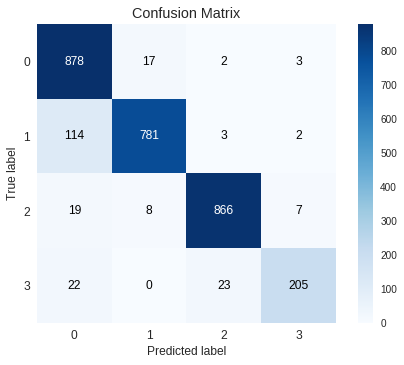
\includegraphics[width=80mm,scale=0.7]{odetestwl.png}
	\caption{Confusion Matrix : first Node model with weighted loss function}
	\label{fig:odetestwl}
\end{figure}
In Fig.~\ref{fig:odetestada} the same model is tested without loss function but using Adasyn.
\begin{figure}[H]  \centering
	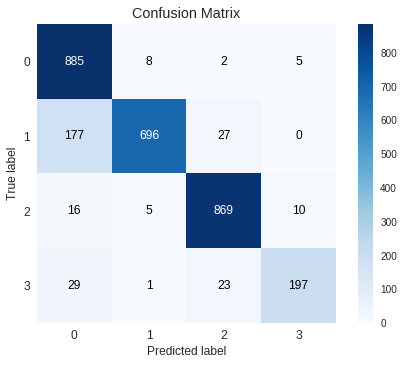
\includegraphics[width=80mm,scale=0.7]{odetestada.png}
	\caption{Confusion Matrix : first Node model with Adasyn}
	\label{fig:odetestada}
\end{figure}
It is clear that weighted loss function performs better than Adasyn: this is due to the first does not create any new samples that may be unrepresentative of the given class. 
\subsection{Test 2}
In this model I have tried to reduce the number of parameters to take full advantages of the parameter efficiency offered by NODE.\\In the previous one, the high number of parameters: 116000, is due to the last fully connected layer that has 32 neurons with an input of size : 3136, for a total of $3136 \cdot 32 = 100352$ parameters.\\In order to reduce the size of the input to this layer that is the output of the ODE block, we have applied a pooling layer in between.\\Specifically, it has a size of 10 and as stride: 5.\\In this case I have used the weighted loss function, since it generally gives better results than Adasyn.\\The number of total parameters is reduced to 34244 that is also less than the CNN of \cite{cnnfazeli} that has 50000 parameters.\\Th results are depicted in fig.~\ref{fig:odelp} 
\begin{figure}[H]  \centering
	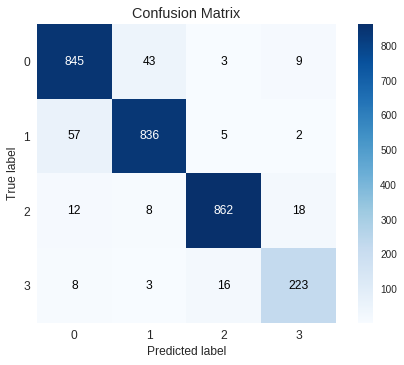
\includegraphics[width=80mm,scale=0.7]{odelp}
	\caption{Confusion Matrix: second Node model with less parameter}
	\label{fig:odelp}
\end{figure}
This model has the best accuracy so far and it is indicative of how a less complex neural network can have better performance.
\subsection{Test 3}
In this case I wanted to check the effect of a de-noise procedure before training the neural network.\\Specifically, I have used the same filtering described in \cite{svmnl}, that consists of the application of DWT to first decompose and later reconstruct the signal. In this case I have used the same model of the first test. The results are depicted in Fig.~\ref{fig:odedwt} and there is an improvement in the accuracy with respect the latter (Fig.~\ref{fig:odetestwl}) 
\begin{figure}[H]  \centering
	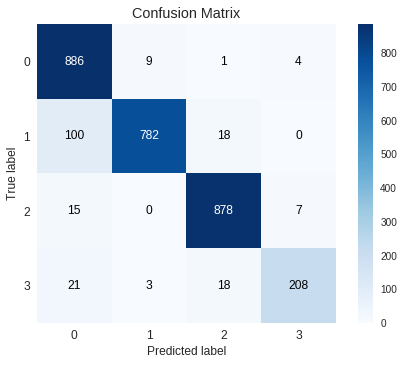
\includegraphics[width=80mm,scale=0.7]{odedwt.png}
	\caption{Confusion Matrix: third model with DWT denoise}
	\label{fig:odedwt}
\end{figure}


\section{LSTM}
In this section, I will describe the application of LSTM for arrhythmia detection. The intuition behind this approach, is to leverage the sequential temporal structure of each beat.\\In fact, the LSTMs have shown great performance for time series, since they can model long term dependency.\\Specifically, for our case, we have that the sequential nature of each beat is crucial for the arrhythmia prediction, because it captures the P wave, QRS complex, ST segment that are essential for the diagnosis.\\We have conducted two main test, that differ in relation to the type of dataset: 
\begin{enumerate}
\item sequences of 200 samples (single beat).
\item sequences of 3/4 beats.
\end{enumerate}
We have tested several model, and in all the circumstances the first configuration had superior performances, and the second one did not reach comparable results neither with the initial algorithm: Random Forest and SVM.\\This is why in the following I will describe only the first case.\\I have implemented all the test below in Keras/TensorFlow, with the following common parameters:
\begin{enumerate}
\item loss function: categorical cross entropy
\item learning rate: 0.001 with exponential decay
\item training epochs: 100
\item Adam optimizer 
\end{enumerate}
Finally, the LSTM's implementation in all the main Python frameworks (Keras, Tensorflow, PyTorch), allows to obtain not only the final hidden state but also the intermediate ones that are crucial if we want to apply attention techniques.\\Specifically, in Keras it is possible to specify an LSTM layer with the following parameters:
\begin{enumerate}
\item \texttt{cell}: each LSTM layer can have multiple cells and each of them outputs a hidden state, for every single element in the input sequence. If no other parameters are specified, the final output of this layer is the last sequence of cell hidden state.
\item \texttt{return\_sequences}: if set to \texttt{True} allows to obtain all the hidden states for each input in the sequence. It is mainly used for applying attention.
\end{enumerate}
The input needs to be three-dimensional with this structure: \texttt{(batch\_size, timesteps, input\_dim)}. The \texttt{timesteps} is always set to 200, while the \texttt{input\_dim} is 1 or 2 with respect to the number of channels we are considering in the original dataset: the ECG signals are recorded with 2 channels.\\In Test 1 and Test 2 we have considered only one channel, while in all the other case both.
\subsection{Test 1}
The neural network has the following structure:
\begin{enumerate}
\item LSTM layer with 32 cells and \texttt{return\_sequences} set to \texttt{True}: the output's shape is \texttt{(batch\_size, timesteps, 32)} 
\item LSTM layer with 32 cells but \texttt{return\_sequences} set to \texttt{False}: the output's shape is \texttt{(batch\_size, 32)} 
\item Dense layer with 4 neurons followed by $softmax$ for the final classification
\end{enumerate}
In Fig.~\ref{fig:lstmt1}, there is the confusion matrix associated to this model. In the following, I will describe more complex approaches.
\begin{figure}[H]  \centering
	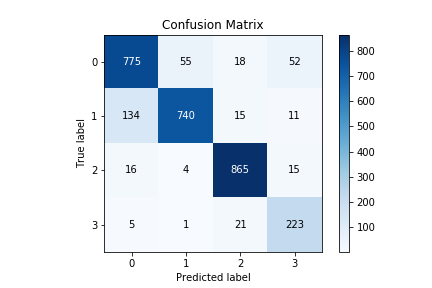
\includegraphics[width=100mm,scale=0.7]{lstmt1}
	\caption{Confusion Matrix: simple model with LSTM}
	\label{fig:lstmt1}
\end{figure}



\subsection{Test 2}
In this case we wanted to build a more elaborated model, with the aim to get better results. We succeed in the latter. However, the drawback is that it has an enormous number of parameters: $1.913.284$
The model is the following:
\begin{enumerate}
\item LSTM layer with 256 cells and \texttt{return\_sequences} set to \texttt{True}: the output's shape is \texttt{(batch\_size, timesteps, 256)} 
\item LSTM layer with 512 cells but \texttt{return\_sequences} set to \texttt{False}: the output's shape is \texttt{(batch\_size, 512)} 
\item Dense layer with 128 neurons followed by $ReLU$
\item Dense layer with 64 neurons followed by $ReLU$
\item Dense layer with 4 neurons followed by $softmax$
\end{enumerate}
In Fig.~\ref{fig:lstmt2}, it is visible the quality of this model in terms of accuracy with respect the previous one, at the expense of a greta number of parameters.
\begin{figure}[H]  \centering
	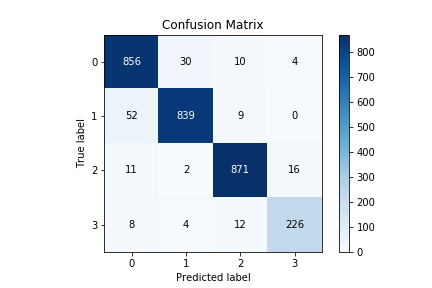
\includegraphics[width=100mm,scale=0.7]{lstmt2}
	\caption{Confusion Matrix: complex model with LSTM}
	\label{fig:lstmt2}
\end{figure}


\subsection{Test 3}
In this case we used both channels so that the input to the model has the shape: texttt{(batch\_size, timesteps, 2)}.\\We have simplified the structure so that it has $822.916$ parameter.\\The model is:
\begin{enumerate}
\item LSTM layer with 256 cells and \texttt{return\_sequences} set to \texttt{True}: the output's shape is \texttt{(batch\_size, timesteps, 256)} 
\item LSTM layer with 256 cells but \texttt{return\_sequences} set to \texttt{False}: the output's shape is \texttt{(batch\_size, 512)} 
\item Dense layer with 128 neurons followed by $ReLU$
\item Dense layer with 4 neurons followed by $softmax$
\end{enumerate}
In Fig.~\ref{fig:lstmt3} we have plotted the results that are better than all the models tried so far.
\begin{figure}[H]  \centering
	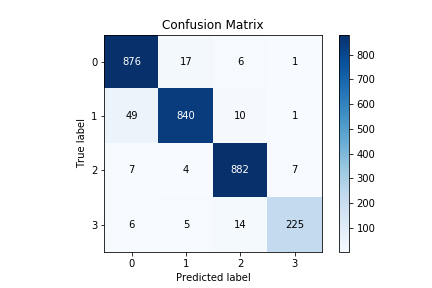
\includegraphics[width=80mm,scale=0.7]{lstmt3}
	\caption{Confusion Matrix: third model with LSTM and 2-D input data}
	\label{fig:lstmt3}
\end{figure}


\section{LSTM/NODE with Attention}
In this section, I will describe how powerful is the application of Attention on the previous models.\\Since our task is a classification problem, namely sequence to one, the decoder state is not present.\\In order to compute the attention score I have taken into consideration the hidden states of the LSTM and as decoder state the last of one, that generally is the value which the decoder state is initialized. Finally, in the following test, we have considered 2 channels for the ECG recording.
Initially, I have adopted Bahdanau's attention on LSTM.\\The neural network is the following:
\begin{enumerate}
\item LSTM layer with 256 cells and \texttt{return\_sequences} set to \texttt{True}: the output's shape is \texttt{(batch\_size, timesteps, 256)} 
\item Bahdanau attention: the output's shape is \texttt{(batch\_size, 256)} 
\item Dense layer with 4 neurons followed by $softmax$
\end{enumerate}
The number of parameters is: $462.597$.
The results are depicted in Fig.~\ref{fig:lstmat1}
\begin{figure}[H]  \centering
	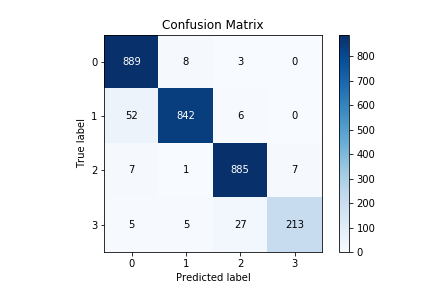
\includegraphics[width=100mm,scale=0.7]{lstmat1}
	\caption{Confusion Matrix: Bahdanau's attention with LSTM}
	\label{fig:lstmat1}
\end{figure}
Secondly, I have used Luong's attention instead of Bahdanau's.\\The results are depicted in Fig.~\ref{fig:lstmat2}.
\begin{figure}[H]  \centering
	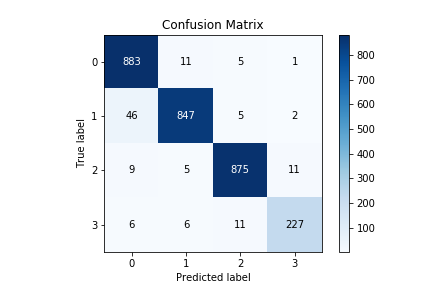
\includegraphics[width=100mm,scale=0.7]{lstmat2}
	\caption{Confusion Matrix: Luong's attention with LSTM}
	\label{fig:lstmat2}
\end{figure}
Next, I have tested the latter model on the dataset with the pre-processing of \cite{cnnfazeli}, with the result in Fig.~\ref{fig:lstmatcnn}. It is interesting to note the pre-processing does not help our models.
\begin{figure}[H]  \centering
	\includegraphics[width=100mm,scale=0.7]{lstmatcnn}
	\caption{Confusion Matrix: Luong's attention with LSTM on the pre-processed dataset of \cite{cnnfazeli}}
	\label{fig:lstmatcnn}
\end{figure}
Finally, I have adopted Luong's attention to the following model that has both a NODE block and LSTM layer. The latter is composed of four principal components: downsampling layers, feature layers, attention layers and fully connected layers.\\The first one is implemented as:
\begin{enumerate}
\item $P_1$: pooling layer of size 5 and stride 2
\item $C_1$,$C_2$: two 1-dimensional convolutional layers with 32 filters, each with padding 5 and stride 2
\item ReLU as activation function
\item the output is: $y_1=P_1(z)$, where $z=ReLU(C_2(ReLU(C_1(x))))$ where $x$ is the original input with 2 channels
\end{enumerate}
The second one is and ODE block with the following parameters:
\begin{enumerate}
\item $C_3$ and $C_4$ are two convolutional layers with the same parameters of $C_2$
\item the output is the ODE function: $y_2=ReLU(C_4(ReLU(C_3(y_1))))$
\end{enumerate}
The third one is where the Luong's attention is applied:
\begin{enumerate}
\item LSTM layer with 128 cells and \texttt{return\_sequences} set to \texttt{True}
\item Luong's attention: the output's shape is \texttt{(batch\_size, 128)} 
\end{enumerate}
Finally the last block is dense layer with 4 neurons followed by $softmax$.
The results are shown below (Fig.~\ref{fig:lstmat3}).
\begin{figure}[H]  \centering
	\includegraphics[width=80mm,scale=0.7]{lstmat3}
	\caption{Confusion Matrix: Luong's attention with LSTM/NODE model}
	\label{fig:lstmat3}
\end{figure}
\section{Transformers}
We have adopted only the encoder part of the Transformers without the decoder, because our task is sequence to one while the latter are used for sequence to many problems.\\The first block is made of:
\begin{enumerate}
\item LSTM layer with 128 cells and \texttt{return\_sequences} set to \texttt{True}
\item Dropout layer with rate: 0.1
\end{enumerate}
Then there are 4 identical layers that implements Multi Head Attention with 4 heads and constitutes the Transformer's Encoder.\\Finally, it is applied, in order:
\begin{enumerate}
\item Dropout layer with rate: 0.1
\item Dense layer with 512 neurons
\item Flatten layer
\item 2 Dense layers with respectively 256 neurons and 4 neurons
\end{enumerate}
It is worth to mention the LSTM layer is necessary to replace the Embedding layer that is originally present in the Transformer.\\However, in our case we could not use the latter because it requires a dictionary of possible values for the input as it is the case of word in input.\\I have also used CNN and the results are the same.
The results are shown below (Fig.~\ref{fig:transf}).
\begin{figure}[H]  \centering
	\includegraphics[width=100mm,scale=0.7]{transf}
	\caption{Confusion Matrix: Transfomers based model }
	\label{fig:transf}
\end{figure}


\section{Per Patient Dataset}
In this part we wanted to check the robustness of the previous models in a more arduous scenario.\\As I explained in the section about the Dataset Configuration, we have removed from the whole dataset: $D$ the following patient's data: $D_{222}$,$D_{223}$,$D_{233}$.\\We have re-trained the LSTM with Loung's attention: $M$ on the remaining data: $D_{train}$, because it is one the best model we have implemented.\\Then we have built a personalized classifier for each of them using two different ways of transfer learning described respectively in Test 1 and Test 2
\subsection{Test 1}
This approach consists of removing the last layer of $M$ so that the latter model can be used as feature extractor.In particular, now the output is a 128 feature vector.\\The we have obtained for each patient's dataset ($D_i$) the corresponding features to train Support Vector Machine with the following parameters:
\begin{enumerate}
\item \texttt{gamma}: 'scale'
\item \texttt{decision\_function\_shape}: 'ovo'
\end{enumerate}
I have used a weighted loss function, but with different weights because the dataset topology in this case is completely different from the previous one.\\In details I have tested several configuration and the best one is provided by \texttt{sklearn}, with the function: \texttt{compute\_class\_weight} and parameters: \texttt{'balanced'}.\\Basically, the weight for each class is assigned in this way: $w_i = \frac{N}{C\cdot f_i}$ where:
\begin{enumerate}
\item $N$: number of samples
\item $C$: number of classes (4)
\item $f_i$: number of beats belong to the $i_{th}$ class
\end{enumerate}
Fig.~\ref{fig:patient222}, Fig.~\ref{fig:patient223}, Fig.~\ref{fig:patient233} , describe respectively the confusion matrix associated to the patients 222,223 and 233.
\begin{figure}[H]  \centering
	\includegraphics[width=100mm,scale=0.7]{patient222}
	\caption{Confusion Matrix for Test 1: Patient 222 }
	\label{fig:patient222}
\end{figure}
\begin{figure}[H]  \centering
	\includegraphics[width=100mm,scale=0.7]{patient223}
	\caption{Confusion Matrix for Test 1: Patient 223 }
	\label{fig:patient223}
\end{figure}
\begin{figure}[H]  \centering
	\includegraphics[width=100mm,scale=0.7]{patient233}
	\caption{Confusion Matrix for Test 1: Patient 233 }
	\label{fig:patient233}
\end{figure}
\subsection{Test 2}
In this part we have fine tuned the original model on each single patient.\\Initially, we have fine tuned all the network's layer.
Fig.~\ref{fig:patient222-transfer-learn}, Fig.~\ref{fig:patient223-transfer-learn}, Fig.~\ref{fig:patient233-transfer-learn} , describe the results.
\begin{figure}[H]  \centering
	\includegraphics[width=100mm,scale=0.7]{patient222-transfer-learn}
	\caption{Confusion Matrix for Test 2 with complete training: Patient 222}
	\label{fig:patient222-transfer-learn}
\end{figure}
\begin{figure}[H]  \centering
	\includegraphics[width=100mm,scale=0.7]{patient223-transfer-learn}
	\caption{Confusion Matrix for Test 2 with complete training: Patient 223}
	\label{fig:patient223-transfer-learn}
\end{figure}
\begin{figure}[H]  \centering
	\includegraphics[width=100mm,scale=0.7]{patient233-transfer-learn}
	\caption{Confusion Matrix for Test 2 with complete training: Patient 233}
	\label{fig:patient233-transfer-learn}
\end{figure}
Finally, we have fine-tuned only the last four layers because the idea is the the initial layers capture general feature about the beat nature.
Fig.~\ref{fig:patient222-transfer-learn-nontrainable}, Fig.~\ref{fig:patient223-transfer-learn-nontrainable}, Fig.~\ref{fig:patient233-transfer-learn-nontrainable} , describe the results.
\begin{figure}[H]  \centering
	\includegraphics[width=100mm,scale=0.7]{patient222-transfer-learn-nontrainable}
	\caption{Confusion Matrix for Test 2 with partial training: Patient 222}
	\label{fig:patient222-transfer-learn-nontrainable}
\end{figure}
\begin{figure}[H]  \centering
	\includegraphics[width=100mm,scale=0.7]{patient223-transfer-learn-nontrainable}
	\caption{Confusion Matrix for Test 2 with partial training: Patient 223}
	\label{fig:patient223-transfer-learn-nontrainable}
\end{figure}
\begin{figure}[H]  \centering
	\includegraphics[width=100mm,scale=0.7]{patient233-transfer-learn-nontrainable}
	\caption{Confusion Matrix for Test 2 with partial training: Patient 233}
	\label{fig:patient233-transfer-learn-nontrainable}
\end{figure}










\chapter{Future Work}















\backmatter
% bibliography
\cleardoublepage
\phantomsection
\bibliographystyle{sapthesis} % BibTeX style
\bibliography{biblio} % BibTeX database without .bib extension

\end{document}
